\myabstract[1]{\vspace{-1cm}\hrule\vspace{2mm}\textbf{Abstract:} Multimodal Retrieval-Augmented Generation (MM-RAG) frequently indexes intermediate textual proxies over raw visual media. Evaluating a 1,626-item multimodal benchmark under frozen 50/50 Dev/Test splits (813 corpus items, 306 test probes), we establish an empirical regime map delineating when text proxies suffice and when native representations are required. On verbatim receipt lookups, character 3--5gram BM25 outperforms word BM25 across OCR engines (Apple Clean: 0.9436 vs.\ 0.8371; Degraded: 0.8248 vs.\ 0.6972; Tesseract 5.5: 0.8412 vs.\ 0.7364; all $p < 10^{-4}$), reversing under entity-substituting light paraphrases (0.2427 vs.\ 0.4334). On document images, document-native ColQwen2 achieves 0.4962 MRR under paraphrasing (+0.0628 over Word BM25, $p = 0.0072$) but shows no statistically significant difference from lexical search on answerable factual questions ($p = 1.0000$). On DocVQA ($N=500$), ColQwen2 (0.6450) substantially outperforms generic text proxies ($\le 0.3507$). Dense bi-encoder deficit is associated with query formulation mismatch rather than sequence truncation; natural answerable questions improve BGE-Base MRR from 0.3256 to 0.5263. On MS-COCO ($N=1{,}000$), native SigLIP retrieval (0.6071) significantly outperforms machine caption proxies (0.3728, $p < 10^{-4}$).
\newline
\newline
\textbf{Keywords:} Multimodal RAG, Text Proxies, Proxy Noise, Dense-Sparse Regime Analysis, Cascade Ranking, Conformal Risk Control, Document Retrieval. \vspace{1mm} \hrule}

\maketitle

\section{Introduction}

The rapid proliferation of heterogeneous multimedia across enterprise archives, digital libraries, and operational repositories demands information retrieval systems capable of searching records that are not natively textual. Transforming scanned documents and images into queryable digital assets is essential for business intelligence, compliance auditing, and decision support \cite{jing2024llmvectordb}. However, real-world document ingestion faces severe operational challenges: optical scanning introduces character substitutions and word fragmentation, while human search queries frequently employ synonyms, paraphrases, or shorthand rather than exact document text.

Retrieval-Augmented Generation (RAG) \cite{lewis2020rag} addresses the hallucination tendencies of Large Language Models (LLMs) by grounding responses in retrieved domain documents. Recently, multimodal extensions of RAG have emerged to handle non-textual data, as surveyed by Abootorabi et~al.~\cite{abootorabi2025multimodal}. For example, Patel et~al.~\cite{patel2025multimodal} and Joshi et~al.~\cite{joshi2024multimodel} presented enterprise multimodal RAG pipelines combining OCR ingestion, multimodal embeddings, and LLM reasoning. Concurrently, native vision-language document retrievers like ColPali \cite{faysse2024colpali} index raw document pixels with multi-vector late interaction.

While foundational studies in information retrieval---notably Kantor and Voorhees~\cite{kantor2000confusion} in the TREC-5 Confusion Track and McNamee and Mayfield~\cite{mcnamee2004character} on character $n$-gram indexing---demonstrated the intrinsic noise resilience of sub-word representations on degraded text, their findings have not been systematically reconciled with modern dense bi-encoders, neural cross-encoder cascades, and document-native vision-language models under semantic query variation. 

To address this gap, this paper establishes \textbf{an empirical regime map of when text proxies suffice versus when native representations are required} across 1,626 multimodal items (scanned receipts, administrative forms, and natural photographs) under frozen 50/50 evaluation splits\footnote{All benchmark collections, evaluation harnesses, and reproduction scripts will be released upon publication at an anonymized repository link [to be provided].}.

\textbf{Key Contributions:}
\begin{enumerate}
    \setlength{\itemsep}{0.2pt plus 0.1pt}
    \setlength{\parskip}{0pt}
    \item \textbf{Sub-Word Inverted Index Dominance and Paraphrase Reversal on Optical OCR:} Evaluating across proprietary Apple Vision \cite{apple2020vision}, open-source Tesseract 5.5 LSTM \cite{smith2007tesseract}, and deep neural EasyOCR 1.7.2 \cite{jaidedai2020easyocr} ($N=306$ held-out probes, 813 corpus items), character 3--5gram BM25 is the single largest sparse architectural lift under verbatim optical noise (+0.1065 clean, +0.1276 degraded blur, +0.1048 clean Tesseract; all $p_{\text{Holm}} < 10^{-4}$). We delineate its strict scope boundary: this advantage reverses under entity-substituting light paraphrases, where Word BM25 outperforms Character BM25 (0.4334 vs.\ 0.2427). On receipts, document-native ColQwen2-v1.0 \cite{faysse2024colqwen2} achieves 0.4962 MRR under paraphrases (+0.0628 over Word BM25, $p_{\text{Holm}} = 0.0072$) but shows no statistically significant difference from lexical search on answerable factual questions (diff $+0.0051$, $p_{\text{Holm}} = 1.0000$) while imposing $286\times$ higher latency (249.21\,ms on Tesla T4 vs.\ 0.87\,ms CPU lookups). Across 500 human-written queries on DocVQA \cite{mathew2021docvqa}, text proxies fed by Tesseract OCR achieve MRR $\le 0.3507$, whereas native ColQwen2 reaches 0.6450 [95\% CI: 0.601, 0.689] (Hit@10 = 84.10\%). We disclose that the ColPali/ColQwen2 architecture incorporates DocVQA training data in its ViDoRe training mixture while text proxies are off-the-shelf; nonetheless, this delineates the visual geometry boundary where native pixels substantially outperform generic text proxies.
    \item \textbf{Dense Bi-Encoder Deficit Governed by Query Formulation:} We demonstrate that dense bi-encoder collapse on document text is associated with single-entity query formulation mismatch rather than sequence truncation constraints (real $\text{max\_seq\_length}=256$; 33.4\% exceed 256 tokens, but chunked MaxP yields identical 0.2030 vs.\ 0.2056 unchunked standard); subword tokenization fragmentation (+122.3\% subwords/word) explains the additional degradation under noise. Formulating queries as natural answerable questions improves BGE-Base MRR from 0.3256 to 0.5263 (Hit@10 79.74\%) on uncorrupted document text without modifying representations. Reconstructing broken tokens via clean Dev lexicon projection recovers $+0.1530$ cosine similarity and $+0.0434$ MRR, providing direct causal evidence for tokenization fragmentation.
    \item \textbf{Native-Visual vs.\ Text-Proxy Representation Boundaries:} On photographic scenes ($N=1{,}000$ MS-COCO Karpathy test images \cite{karpathy2015deep, lin2014coco}), native visual embeddings (SigLIP Base Patch16 MRR = 0.6071 \cite{zhai2023siglip}) significantly outperform machine caption proxies (MiniLM MRR = 0.3728 \cite{reimers2019sbert}, $p < 10^{-4}$), showing that synthetic captions lose essential visual nuance, with no statistically significant difference detected from human gold captions (diff $-0.0236$, $p=0.142$, equivalence not asserted). In contrast, for document pages, text proxies suffice when queries contain lexical anchors.
    \item \textbf{Actionable Empirical Decision Guide for MM-RAG Builders:} We synthesize our experimental findings across OCR engines, degradation levels, and query formulations into an empirical decision guide, detailing optimal retrieval architectures and statistically indistinguishable sets across document, image, and query regimes.
\end{enumerate}

\section{Related Work}
\label{sec:related_work}

\subsection{Multimodal Representation and Retrieval}
Early cross-modal retrieval systems relied on dual-encoder contrastive learning. Models like CLIP \cite{radford2021clip} and SigLIP \cite{zhai2023siglip} project images and text into a shared latent space using sigmoid or softmax cross-entropy objectives. ImageBind \cite{girdhar2023imagebind} extended this paradigm across six modalities using images as the central binding modality. While effective for broad semantic matching, dual-encoders compress multimedia into fixed-dimension vectors, frequently losing granular lexical and structural tokens. Our hybrid design combines dense embeddings with sparse lexical representations such as BM25 \cite{robertson2009bm25, robertson1995okapi} to retain both semantic intent and exact token matches.

\subsection{Multimodal RAG and Document Analysis}
Integrating multimodal inputs into RAG workflows has advanced rapidly with Vision-Language Models (VLMs) and document foundation models. Document retrievers such as ColPali \cite{faysse2024colpali} and M3DocRAG \cite{cho2024m3docrag}, benchmarked on the ViDoRe suite \cite{faysse2024colpali} and DocVQA \cite{mathew2021docvqa}, index document pages using multi-vector vision-language representations (e.g., Qwen2-VL \cite{wang2024qwen2vl}) to bypass OCR. A paradigm comparison is presented in Table~\ref{tab:sota_comparison}. While promising, multi-vector representations require substantial GPU memory and cross-attention compute. Conversely, enterprise systems \cite{patel2025multimodal, joshi2024multimodel} mediate retrieval through text proxies. Our work evaluates this trade-off: systematically delineating where text proxies excel and where native visual representations remain necessary.



\subsection{Character Subwords and OCR Degradation in Information Retrieval}
Optical Character Recognition (OCR) systems translate document imagery into text, but routinely introduce character substitutions, insertions, deletions, and bounding-box permutations \cite{smith2007tesseract, fateh2024ocr}. Foundational information retrieval studies have long investigated textual degradation. In the TREC-5 Confusion Track, Kantor and Voorhees~\cite{kantor2000confusion} systematically evaluated retrieval on scanned, OCR-corrupted collections (at 5\% and 20\% error rates), establishing known-item retrieval benchmarks under optical corruption. Complementing this, McNamee and Mayfield~\cite{mcnamee2004character} established that overlapping character $n$-gram tokenization (e.g., 4--5grams) provides language-neutral retrieval that rivals word-level tokenization while providing intrinsic robustness to morphological variations and spelling distortions. Early image-domain mitigation strategies, including Otsu thresholding \cite{otsu1979} and Hough transforms \cite{hough1962} for skew correction, focused on image-domain preprocessing. Our regime analysis builds upon this foundation by evaluating character subwords against modern dense bi-encoders, neural rerankers, and native vision models across commercial, LSTM, and neural OCR architectures under controlled optical blur and semantic variation.

\begin{table*}[t]
\centering
\small
\caption{Systematic Comparison with Prior Multimodal Information Retrieval and RAG Frameworks.}
\label{tab:sota_comparison}
\resizebox{\textwidth}{!}{%
\begin{tabular}{@{}lcccccc@{}}
\toprule
\textbf{System / Architecture} & \textbf{Publication Venue} & \textbf{Document Retrieval} & \textbf{Natural Image Retrieval} & \textbf{Multi-Hop Mechanism} & \textbf{Benchmark Datasets} & \textbf{Hardware Serving Profile} \\ \midrule
ColPali \cite{faysse2024colpali} & ICLR 2025 & nDCG@5 = 0.813 (ViDoRe) & Supported (Multi-Vector) & Single-pass only & ViDoRe Benchmark & Multi-GPU ($\ge 16$\,GB VRAM, $\sim$250\,ms) \\
M3DocRAG \cite{cho2024m3docrag} & EMNLP 2024 & QA Acc.\ 64.2\% (MP-DocVQA) & Supported (Dense VLM) & Generative LLM bridging & MP-DocVQA, DUDE & High-End GPU Cluster ($\ge 48$\,GB VRAM) \\
Patel et~al. \cite{patel2025multimodal} & IEEE ETCC 2025 & Heuristic OCR matching & ImageBind vector search & Single-pass only & Proprietary enterprise text/media & Dedicated GPU Server \\
Baleen \cite{khattab2021baleen} & NeurIPS 2021 & Not evaluated (Text QA) & Not supported & Generative condensed hops & HotpotQA (Text only) & GPU / High-RAM CPU Server \\
\textbf{Proposed Regime Framework} & \textbf{This Work} & \textbf{MRR 0.9436 (Char BM25)} & \textbf{MRR 0.6071 (SigLIP Pixels)} & \textbf{Exploratory PRF (Hit@10 0.640, $N=50$, Sec.~VI-B)} & \textbf{SROIE, FUNSD, MS-COCO, DocVQA} & \textbf{CPU char BM25 ($<1$\,ms verbatim) / Cross-Encoder Cascade} \\ \bottomrule
\end{tabular}}
\vspace{1mm}\newline
\raggedright\scriptsize Note: Qualitative columns reflect architectural design choices; our reported MRR and Hit@10 figures are from held-out evaluation on SROIE/FUNSD/COCO/DocVQA and are not directly comparable to other systems' proprietary benchmarks. Table~\ref{tab:sota_comparison} is a qualitative paradigm map, not a cross-system numerical comparison. ColPali and M3DocRAG figures are from their respective original papers.
\end{table*}

\subsection{Modern Dense and Learned Sparse Retrieval Models}
Dense bi-encoders encode queries and passages independently \cite{reimers2019sbert, xiao2023bge}. Recent architectures have expanded this paradigm: multilingual dense models such as BGE-M3 \cite{chen2024bgem3} support multi-granularity representations; learned sparse models like SPLADE \cite{formal2021splade} expand queries and documents into vocabulary-space term weights; and late-interaction multi-vector architectures like ColBERTv2 \cite{santhanam2022colbertv2} preserve token-level interactions at reduced latency. We position standard bi-encoders (\texttt{all-MiniLM-L6-v2}, \texttt{bge-base-en-v1.5}) and late-interaction vision models (\texttt{ColQwen2-v1.0}) within this broader landscape.

\subsection{Cascade Ranking and Conformal Risk Control}
Cascade ranking architectures \cite{wang2011cascade, gallagher2019cascade} balance retrieval efficiency and precision by passing candidates through tiered stages, escalating to expressive models only when scores indicate ranking ambiguity. Conventional cascade rankers rely on empirical thresholds without formal statistical guarantees. Conformal prediction, formulated by Bates et~al.~\cite{bates2021conformal} and surveyed by Angelopoulos and Bates~\cite{angelopoulos2021gentle}, provides a distribution-free, finite-sample framework for bounding user-specified risk metrics below a tolerance $\alpha$. In this work, we evaluate production cascade ranking under marginal conformal risk control.

\section{Reference Retrieval Architecture}
\label{sec:architecture}

\begin{figure*}[t]
\centering
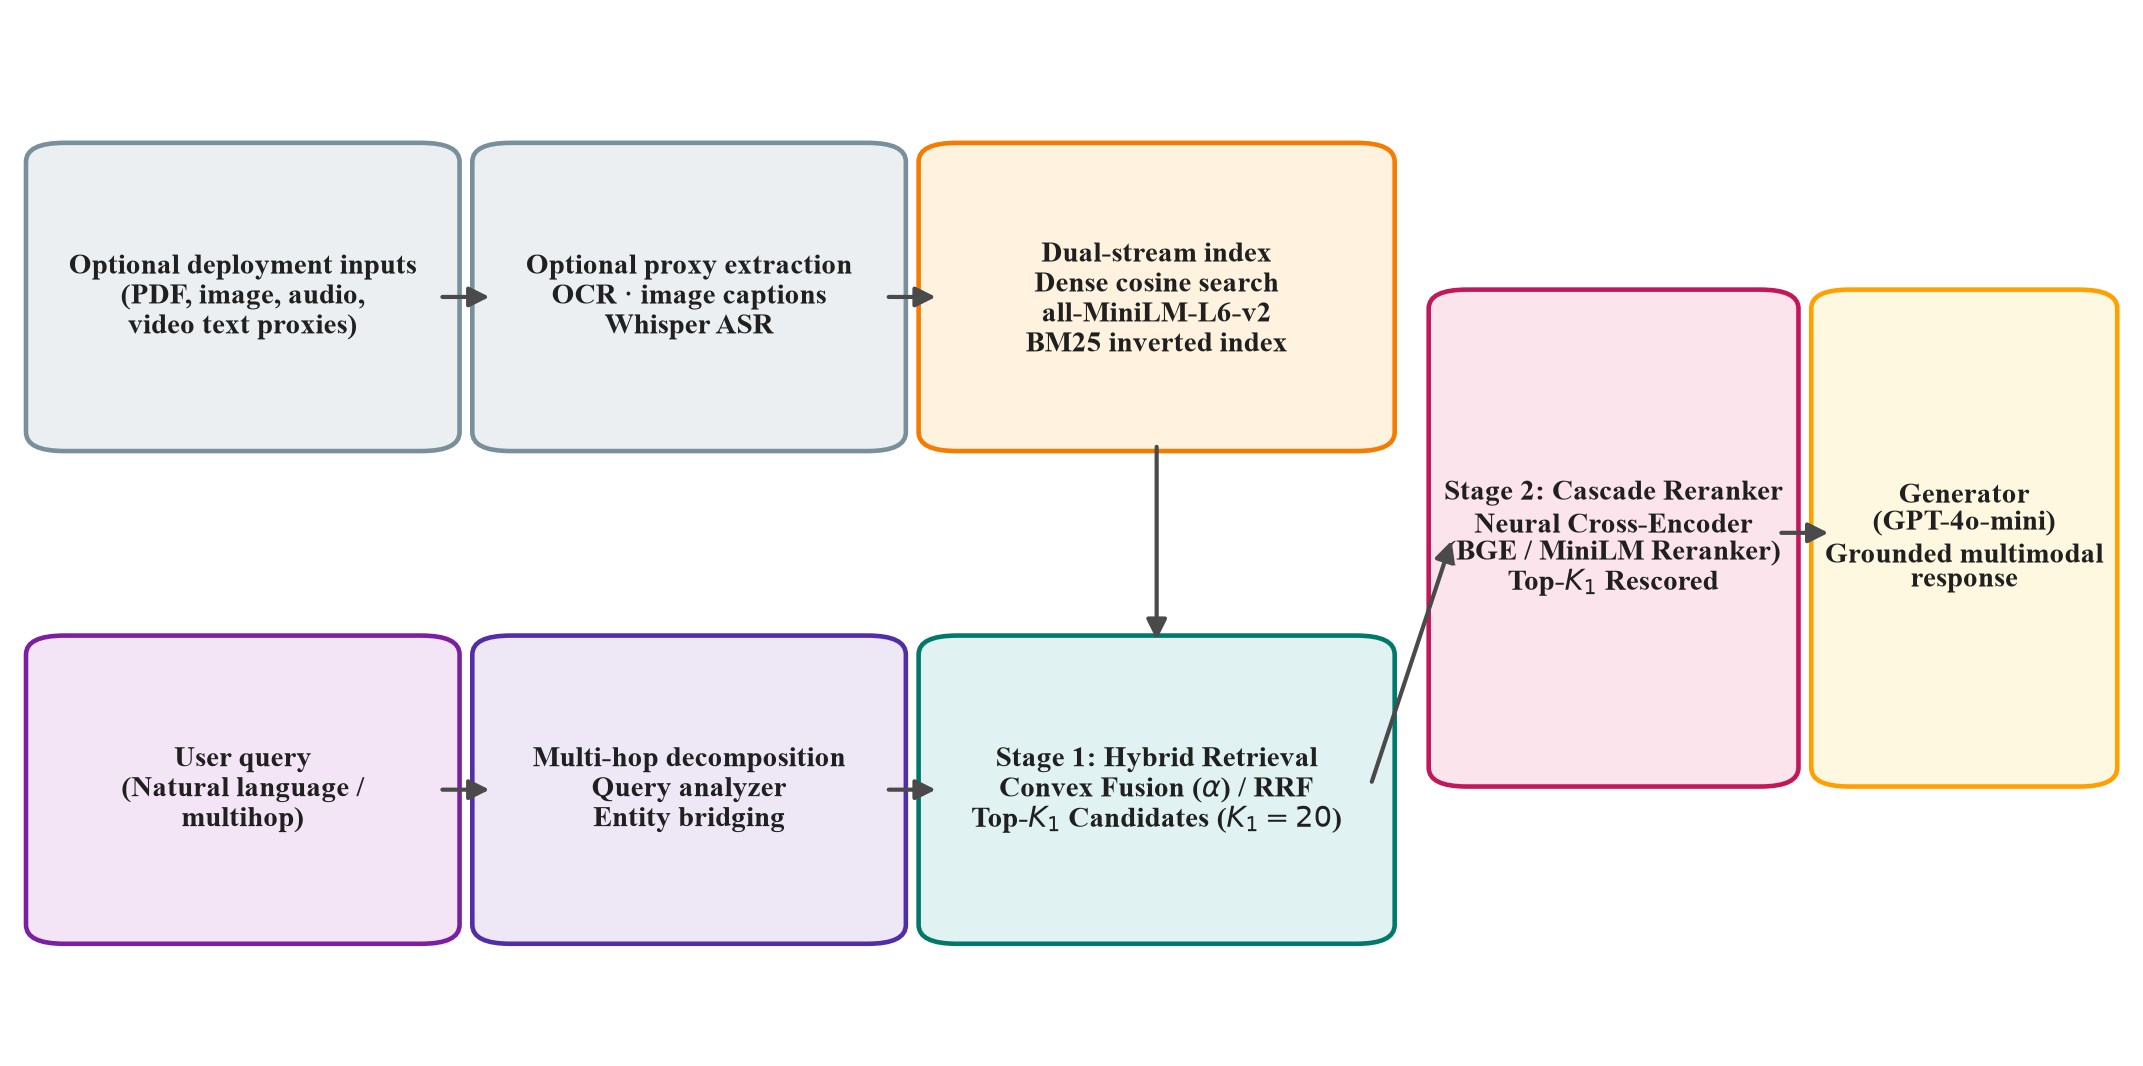
\includegraphics[width=0.82\textwidth]{figures/fig_architecture.png}
\caption{Conceptual reference architecture of the text-proxy RAG framework. Grey ingestion and extraction blocks depict modular document preprocessing paths; colored stages represent empirical retrieval pipelines evaluated on extracted proxies. Un-evaluated production extensions (e.g., dual-signal router, conformal gate) are ablated in Section~\ref{sec:negative_findings}.}
\label{fig:architecture}
\end{figure*}

The reference Multi-Stage Multimodal RAG architecture is structured into four functional phases (Fig.~\ref{fig:architecture}): (1) Ingestion and Preprocessing, (2) Hybrid Dense-Sparse First-Stage Retrieval, (3) Neural Cross-Encoder Reranking and Cascade Escalation, and (4) Context Assembly.

\subsection{Ingestion and Preprocessing Pipeline}
Unstructured enterprise multimedia are mediated through textual proxies. Proxies can be extracted across modalities via OCR text \cite{smith2007tesseract}, vision-language captions \cite{li2022blip, li2023blip2, xiao2024florence2}, and speech transcripts \cite{radford2023whisper}.
\begin{itemize}
    \setlength{\itemsep}{0.2pt plus 0.1pt}
    \setlength{\parskip}{0pt}
    \item \textbf{Documents and Forms:} Administrative forms and receipts are processed through document decomposition, optional Otsu binarization \cite{otsu1979} and Hough skew correction \cite{hough1962}, extracting text $T_d$ and bounding boxes via OCR engines (Apple Vision \cite{apple2020vision}, Tesseract 5.5 \cite{smith2007tesseract}, or EasyOCR \cite{jaidedai2020easyocr}).
    \item \textbf{Photographs:} Natural photographs are indexed via machine captions alongside native visual embeddings (CLIP \cite{radford2021clip}, SigLIP \cite{zhai2023siglip}).
    \item \textbf{Acoustic Media:} Continuous audio is transcribed using Whisper \cite{radford2023whisper} or embedded using contrastive audio representations (CLAP \cite{wu2023clap}).
\end{itemize}

Dense embeddings are generated via Sentence-BERT (\texttt{all-MiniLM-L6-v2}) \cite{reimers2019sbert} and BGE (\texttt{bge-base-en-v1.5}) \cite{xiao2023bge}, while lexical tokens are indexed with BM25 \cite{robertson2009bm25, robertson1995okapi}. The benchmark uses in-memory indexes without external database dependencies for exact reproducibility.

\subsection{Stage 1: Hybrid Dense-Sparse Retrieval}
Given query $q$, single-stage dense retrieval computes vector similarity:
\begin{equation}
    S_{\text{dense}}(q, d) = \cos(\mathbf{e}_q^{\text{dense}}, \mathbf{e}_d^{\text{dense}}) = \frac{\mathbf{e}_q \cdot \mathbf{e}_d}{\|\mathbf{e}_q\| \|\mathbf{e}_d\|}
\end{equation}
While effective for thematic alignment, dense retrieval often overlooks exact alphanumeric codes. Conversely, sparse BM25 retrieval excels at lexical precision:
\begin{equation}
    S_{\text{sparse}}(q, d) = \sum_{t \in q} \text{IDF}(t) \cdot \frac{f(t, d) \cdot (k_1 + 1)}{f(t, d) + k_1 \cdot \left(1 - b + b \cdot \frac{|d|}{\text{avgdl}}\right)}
\end{equation}
We evaluate Normalized Convex Combination ($S_{\text{hybrid}} = \alpha \hat{S}_{\text{dense}} + (1-\alpha) \hat{S}_{\text{sparse}}$) and Reciprocal Rank Fusion (RRF) \cite{cormack2009rrf}:
\begin{equation}
    \text{RRF}(q, d) = \frac{1}{k + r_{\text{dense}}(d)} + \frac{1}{k + r_{\text{sparse}}(d)}
    \label{eq:rrf}
\end{equation}
with $k=60$. First-stage candidate depth is set to $K_1 = 20$.

\subsection{Stage 2: Candidate Reranking via Neural Cross-Encoders}
Bi-encoders compute query and document representations independently. To recover joint attention, Stage~2 deploys a pretrained neural cross-encoder (\texttt{BAAI/bge-reranker-base} \cite{xiao2023bge} or \texttt{ms-marco-MiniLM-L-6-v2} \cite{reimers2019sbert}) to rescore the top-$K_1$ candidates ($K_1 = 20$):
\begin{equation}
    S_{\text{rerank}}(q, d) = \text{CrossEncoder}(q, d)
\end{equation}
Scoring every candidate pool with a cross-encoder adds latency. We evaluate confidence-margin cascades ($\Delta_{1,2} = s^{(1)} - s^{(2)} < \tau$) and marginal conformal risk control to escalate only ambiguous queries.

\section{Experimental Setup}
\label{sec:experimental_setup}

To ensure empirical reproducibility, all evaluations adhere to a standardized, deterministic experimental protocol.

\subsection{Datasets and Split Partitions}
Our benchmark evaluates 1,626 pooled multimodal items:
\begin{itemize}
    \setlength{\itemsep}{0.2pt plus 0.1pt}
    \setlength{\parskip}{0pt}
    \item \textbf{SROIE Receipts \cite{huang2019sroie}:} 626 scanned retail receipts from the ICDAR 2019 competition, comprising 612 factual probes.
    \item \textbf{MS-COCO Images \cite{lin2014coco}:} 1,000 photographic distractor images and held-out human descriptions evaluated under the Karpathy test split \cite{karpathy2015deep}.
    \item \textbf{FUNSD Administrative Forms \cite{jaume2019funsd}:} 100 scanned business forms with rich multi-field tabular structures and 600 distractor forms.
    \item \textbf{DocVQA Benchmark \cite{mathew2021docvqa}:} 500 document images and 500 100\% human-authored questions from the ViDoRe benchmark collection \cite{faysse2024colpali}.
\end{itemize}
To prevent data snooping, SROIE is partitioned into a strict 50/50 Dev/Test split by Item ID ($N=306$ probes, 813 corpus items each). The Dev split is dedicated strictly to hyperparameter tuning (e.g., fusion $\alpha^*$, conformal thresholds $\tau^*$). The Test split is frozen for evaluation across Seeds 42, 43, and 44 with zero test tuning.

\subsection{OCR Engines and Optical Degradation Conditions}
Document text is extracted across three distinct OCR engines:
\begin{enumerate}
    \setlength{\itemsep}{0.2pt plus 0.1pt}
    \setlength{\parskip}{0pt}
    \item \textbf{Apple Vision Neural OCR \cite{apple2020vision}:} Commercial neural OCR (\texttt{VNRecognizeTextRequest}).
    \item \textbf{Tesseract 5.5 LSTM OCR \cite{smith2007tesseract}:} Standard open-source LSTM OCR engine.
    \item \textbf{EasyOCR 1.7.2 Deep CRNN \cite{jaidedai2020easyocr}:} Deep neural OCR combining CRAFT text detection and ResNet-CRNN recognition.
\end{enumerate}
Documents are evaluated under: (1)~\emph{Clean OCR}, (2)~\emph{Realistic Optical Degradation} (Gaussian blur $\sigma=1.5$, bilinear 50\% downscaling, random skew $\pm 2.5^\circ$, JPEG compression $Q=20$), and (3)~\emph{Human Ground Truth} text.

\subsection{Unified Query Slices}
To isolate semantic abstraction from optical noise, queries are structured into four canonical slices:
\begin{enumerate}
    \setlength{\itemsep}{0.2pt plus 0.1pt}
    \setlength{\parskip}{0pt}
    \item \textbf{Verbatim Lookups:} Exact textual substrings extracted from documents (100\% token overlap), representing known-item search.
    \item \textbf{Light Paraphrases:} Lexical substitutions and entity rewrites (41.2\% mean token overlap; e.g., substituting ``dinner bill'' for ``total payable''), testing semantic abstraction.
    \item \textbf{Answerable Factual Questions:} Natural interrogatives preserving key factual and topical anchors (e.g., ``What was the total payment at Book Ta K?''), testing real-world question answering.
    \item \textbf{Legacy Token-Stripped Probes:} Probes where shared lexical tokens are deliberately removed, used strictly for conformal risk stress-testing.
\end{enumerate}
Unless noted otherwise, evaluation queries for SROIE and FUNSD were synthesized using \texttt{gpt-4o-mini} \cite{openai2024gpt4o} at temperature $T=0.0$. DocVQA queries are 100\% human-authored.

\subsection{Candidate Retrieval Systems}
We benchmark: (1) Word BM25 \cite{robertson2009bm25}; (2) Character 3--5gram BM25 \cite{mcnamee2004character}; (3) Dense MiniLM (\texttt{all-MiniLM-L6-v2}) \cite{reimers2019sbert}; (4) Dense BGE-Base (\texttt{bge-base-en-v1.5}) \cite{xiao2023bge}; (5) Dev-Tuned Hybrid (normalized convex fusion); (6) Neural Cross-Encoders (\texttt{bge-reranker-base} \cite{xiao2023bge}, \texttt{ms-marco-MiniLM-L-6-v2} \cite{reimers2019sbert}); (7) Document-Native ColQwen2-v1.0 \cite{faysse2024colqwen2}; and (8) Vision Encoders (CLIP ViT-B/32 \cite{radford2021clip}, SigLIP Base Patch16 \cite{zhai2023siglip}).

\subsection{Evaluation Metrics and Statistical Testing}
Systems are evaluated on Mean Reciprocal Rank (MRR), Hit@k ($k \in \{1, 5, 10\}$), and nDCG@10. Paired differences are evaluated via two-tailed paired permutation tests ($N_{\text{perm}}=100{,}000$ sign flips) with Holm-Bonferroni correction ($p_{\text{Holm}}$). Confidence intervals (95\% CI) are computed via cluster bootstrap resampling at the document level (10,000 iterations).

\subsection{Hardware Serving Profiles}
Sparse BM25 and bi-encoders are profiled on Apple M2 (16\,GB RAM, batch size = 1, warm cache). Neural cross-encoders and ColQwen2 are profiled on Nvidia Tesla T4 GPU (14.56\,GB VRAM, batch size = 1, warm cache).

\section{Empirical Regime Analysis and Results}
\label{sec:results}

\subsection{Regime A: Text-Dominated Document and Receipt Retrieval}
\label{sec:regime_a_text}

Table~\ref{tab:regime_grid_v3} presents retrieval effectiveness across systems, query formulations, and noise regimes on the held-out test split ($N=306$). In Table~\ref{tab:regime_grid_v3}, the 500 COCO distractors have their ground-truth caption text indexed as fallback (yielding Word BM25 0.8371, Char BM25 0.9436, Ground Truth 0.9853 on verbatim; Word BM25 0.4334 on light paraphrase). In the receipt-only distractor pool of Table~\ref{tab:engine_replication_v3}, unannotated distractors are left as empty text (yielding Word BM25 0.8324, Char BM25 0.9443, Ground Truth 0.9854 on verbatim; Word BM25 0.4003 on light paraphrase).

\begin{table*}[t]
\centering
\small
\caption{Multimodal Text-Proxy Retrieval Regime Analysis across Query Types and Noise Regimes (Held-Out Public Test Split, $N=306$ Probes, 813 Distractor Pool, 95\% Cluster Bootstrap CIs). Dense MiniLM/BGE latencies (0.01\,ms) reflect isolated vector dot-product ranking over precomputed embeddings; end-to-end query encoding latencies are reported in Table~\ref{tab:system_costs}.}
\label{tab:regime_grid_v3}
\resizebox{\textwidth}{!}{%
\begin{tabular}{llccccc}
\toprule
Query Type & Retrieval System & Clean MRR [95\% CI] & Syn 20\% MRR [95\% CI] & Real-OCR MRR [95\% CI] & Optical Blur MRR [95\% CI] & Latency (ms) \\
\midrule
\multirow{7}{*}{\textbf{Verbatim}}
 & BM25 (Tuned)            & 0.8572 [0.822, 0.890] & 0.3961 [0.364, 0.429] & 0.8371 [0.798, 0.871] & 0.6972 [0.650, 0.741] & 0.13 \\
 & BM25 (Char 3-5gram)     & 0.9853 [0.972, 0.995] & 0.7252 [0.694, 0.757] & 0.9436 [0.919, 0.965] & 0.8248 [0.782, 0.864] & 0.87 \\
 & Dense MiniLM (unchunked) & 0.2100 [0.171, 0.252] & 0.0596 [0.045, 0.077] & 0.2056 [0.166, 0.247] & 0.1724 [0.135, 0.210] & 0.01 \\
 & Dense BGE-base (unchunked)& 0.3256 [0.276, 0.376] & 0.1347 [0.109, 0.162] & 0.3022 [0.256, 0.351] & 0.2471 [0.202, 0.292] & 0.01 \\
 & Tuned Hybrid            & 0.8572 [0.822, 0.890] & 0.3979 [0.365, 0.431] & 0.8367 [0.798, 0.871] & 0.6940 [0.646, 0.739] & 0.13 \\
 & CLIP Visual             & 0.0436 [0.028, 0.062] & 0.0436 [0.028, 0.062] & 0.0436 [0.028, 0.062] & 0.0436 [0.028, 0.062] & 12.50 \\
 & Uniform Random Ranking  & 0.0089 [0.009, 0.009] & 0.0089 [0.009, 0.009] & 0.0089 [0.009, 0.009] & 0.0089 [0.009, 0.009] & 0.01 \\
\midrule
\multirow{7}{*}{\textbf{Light Paraphrase}}
 & BM25 (Tuned)            & 0.4790 [0.427, 0.530] & 0.1394 [0.118, 0.162] & 0.4334 [0.380, 0.484] & 0.3630 [0.315, 0.412] & 0.08 \\
 & BM25 (Char 3-5gram)     & 0.2504 [0.209, 0.290] & 0.1295 [0.105, 0.155] & 0.2427 [0.202, 0.282] & 0.2137 [0.178, 0.252] & 2.53 \\
 & Dense MiniLM (unchunked)  & 0.1230 [0.092, 0.155] & 0.0371 [0.027, 0.049] & 0.1086 [0.080, 0.139] & 0.0772 [0.054, 0.103] & 0.01 \\
 & Dense BGE-base (unchunked)& 0.1670 [0.131, 0.205] & 0.0684 [0.051, 0.086] & 0.1601 [0.124, 0.197] & 0.1275 [0.096, 0.161] & 0.01 \\
 & Tuned Hybrid            & 0.4572 [0.408, 0.507] & 0.1445 [0.125, 0.166] & 0.4335 [0.382, 0.483] & 0.3657 [0.318, 0.413] & 0.08 \\
 & CLIP Visual             & 0.0303 [0.020, 0.042] & 0.0303 [0.020, 0.042] & 0.0303 [0.020, 0.042] & 0.0303 [0.020, 0.042] & 12.50 \\
 & Uniform Random Ranking  & 0.0089 [0.009, 0.009] & 0.0089 [0.009, 0.009] & 0.0089 [0.009, 0.009] & 0.0089 [0.009, 0.009] & 0.01 \\
\midrule
\multirow{7}{*}{\textbf{Answerable Questions}}
 & BM25 (Tuned)            & 0.9116 [0.885, 0.937] & 0.4042 [0.370, 0.440] & 0.9014 [0.873, 0.929] & 0.7328 [0.688, 0.773] & 0.60 \\
 & BM25 (Char 3-5gram)     & 0.9653 [0.947, 0.982] & 0.6270 [0.592, 0.662] & 0.9471 [0.923, 0.969] & 0.8116 [0.770, 0.848] & 5.72 \\
 & Dense MiniLM (unchunked)  & 0.3669 [0.323, 0.414] & 0.1061 [0.089, 0.125] & 0.2837 [0.241, 0.328] & 0.2260 [0.190, 0.265] & 0.01 \\
 & Dense BGE-base (unchunked)& 0.5197 [0.475, 0.566] & 0.2005 [0.175, 0.228] & 0.5128 [0.468, 0.560] & 0.4313 [0.386, 0.479] & 0.02 \\
 & Tuned Hybrid            & 0.8084 [0.768, 0.844] & 0.4120 [0.376, 0.450] & 0.7705 [0.728, 0.811] & 0.5346 [0.486, 0.579] & 0.61 \\
 & CLIP Visual             & 0.0388 [0.024, 0.057] & 0.0388 [0.024, 0.057] & 0.0388 [0.024, 0.057] & 0.0388 [0.024, 0.057] & 12.50 \\
 & Uniform Random Ranking  & 0.0089 [0.009, 0.009] & 0.0089 [0.009, 0.009] & 0.0089 [0.009, 0.009] & 0.0089 [0.009, 0.009] & 0.01 \\
\bottomrule
\end{tabular}}
\end{table*}

\begin{figure}[t]
\centering
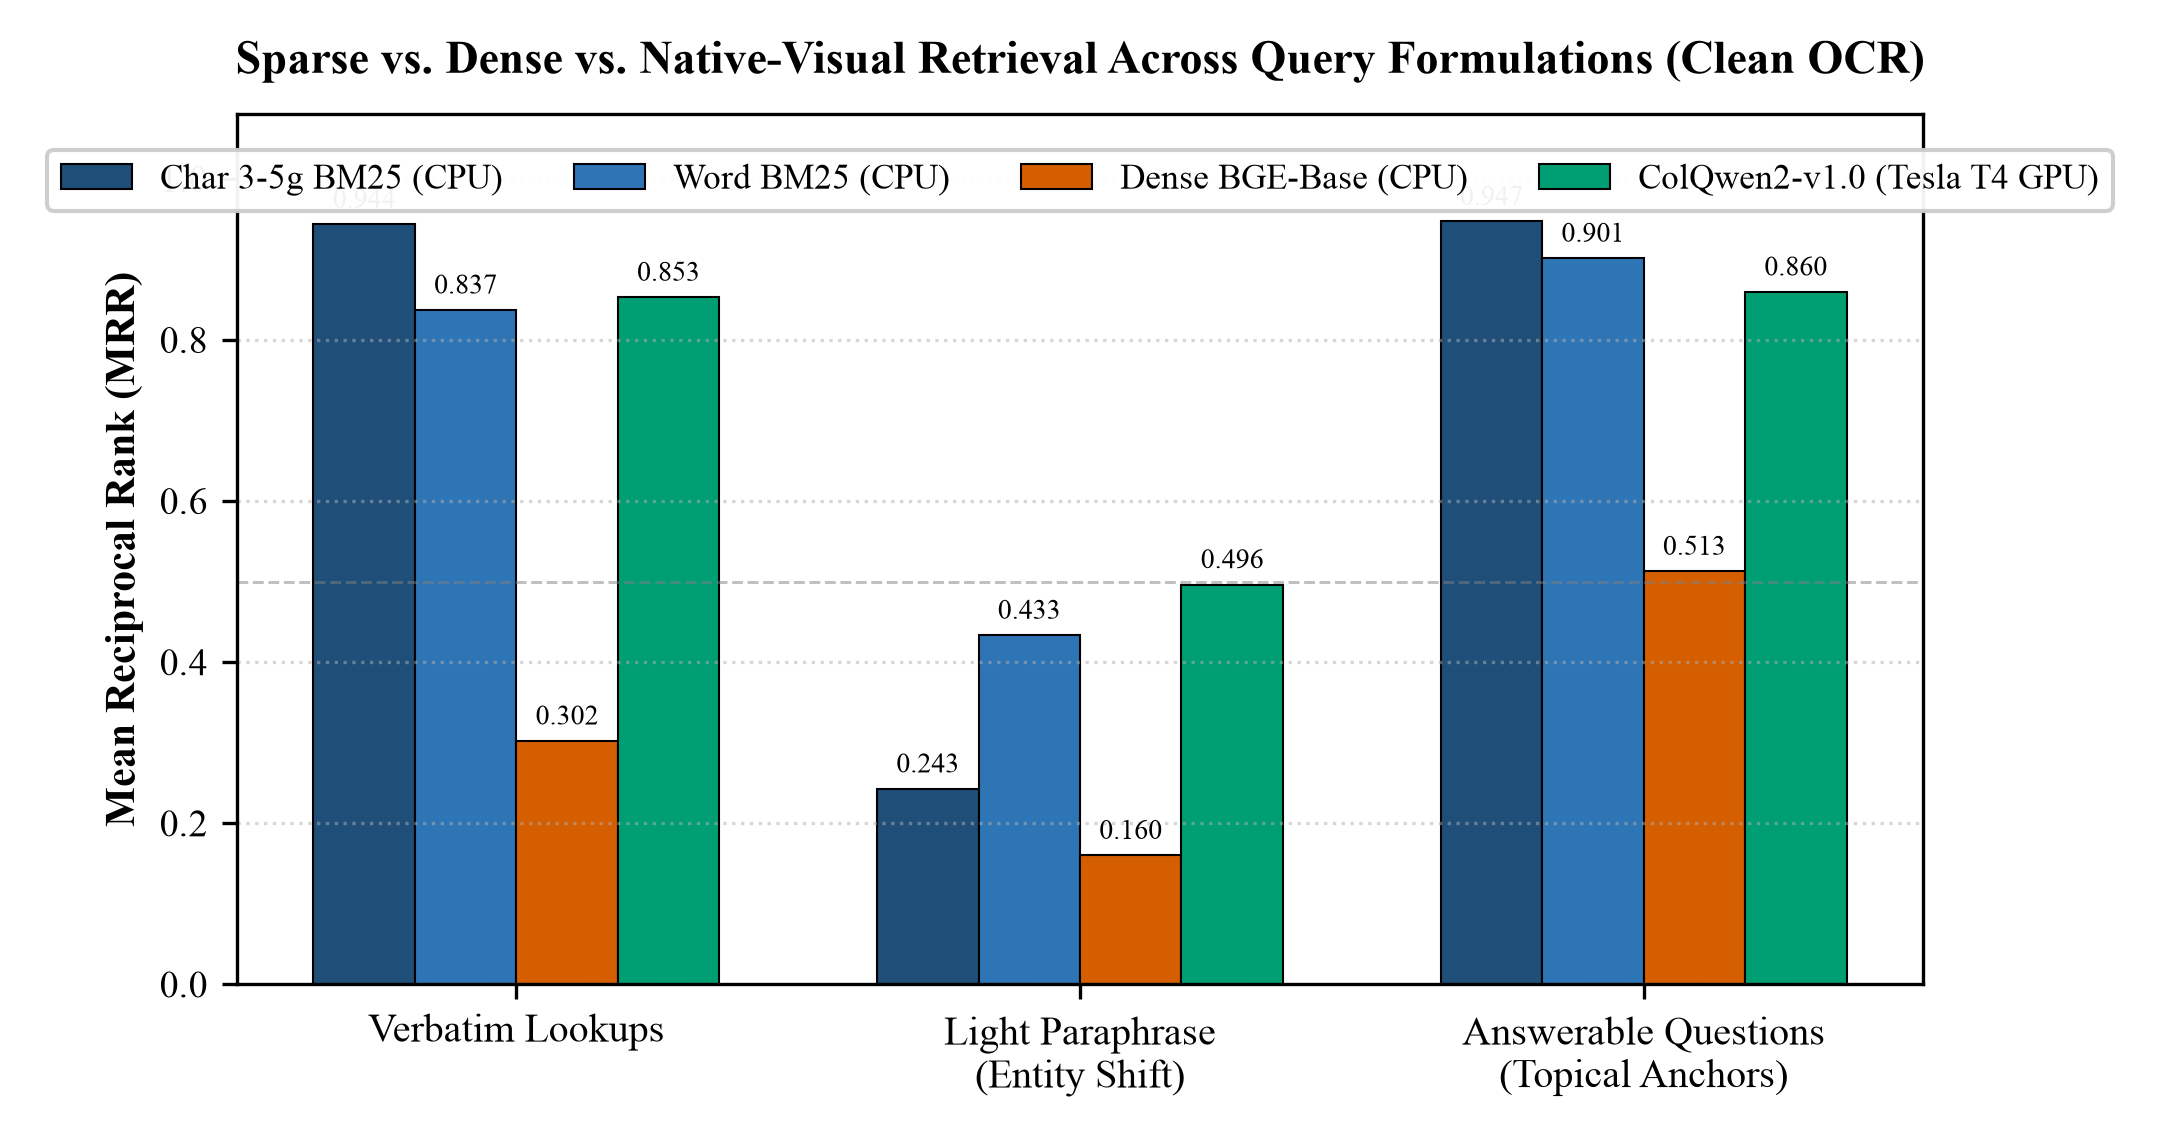
\includegraphics[width=0.80\columnwidth]{figures/fig_mrr_regime_systems.png}
\caption{Retrieval effectiveness (MRR@10 with 95\% bootstrap error bars) across retrieval architectures and query formulations on clean receipt OCR.}
\label{fig:mrr_regime_systems}
\end{figure}

\begin{figure}[t]
\centering
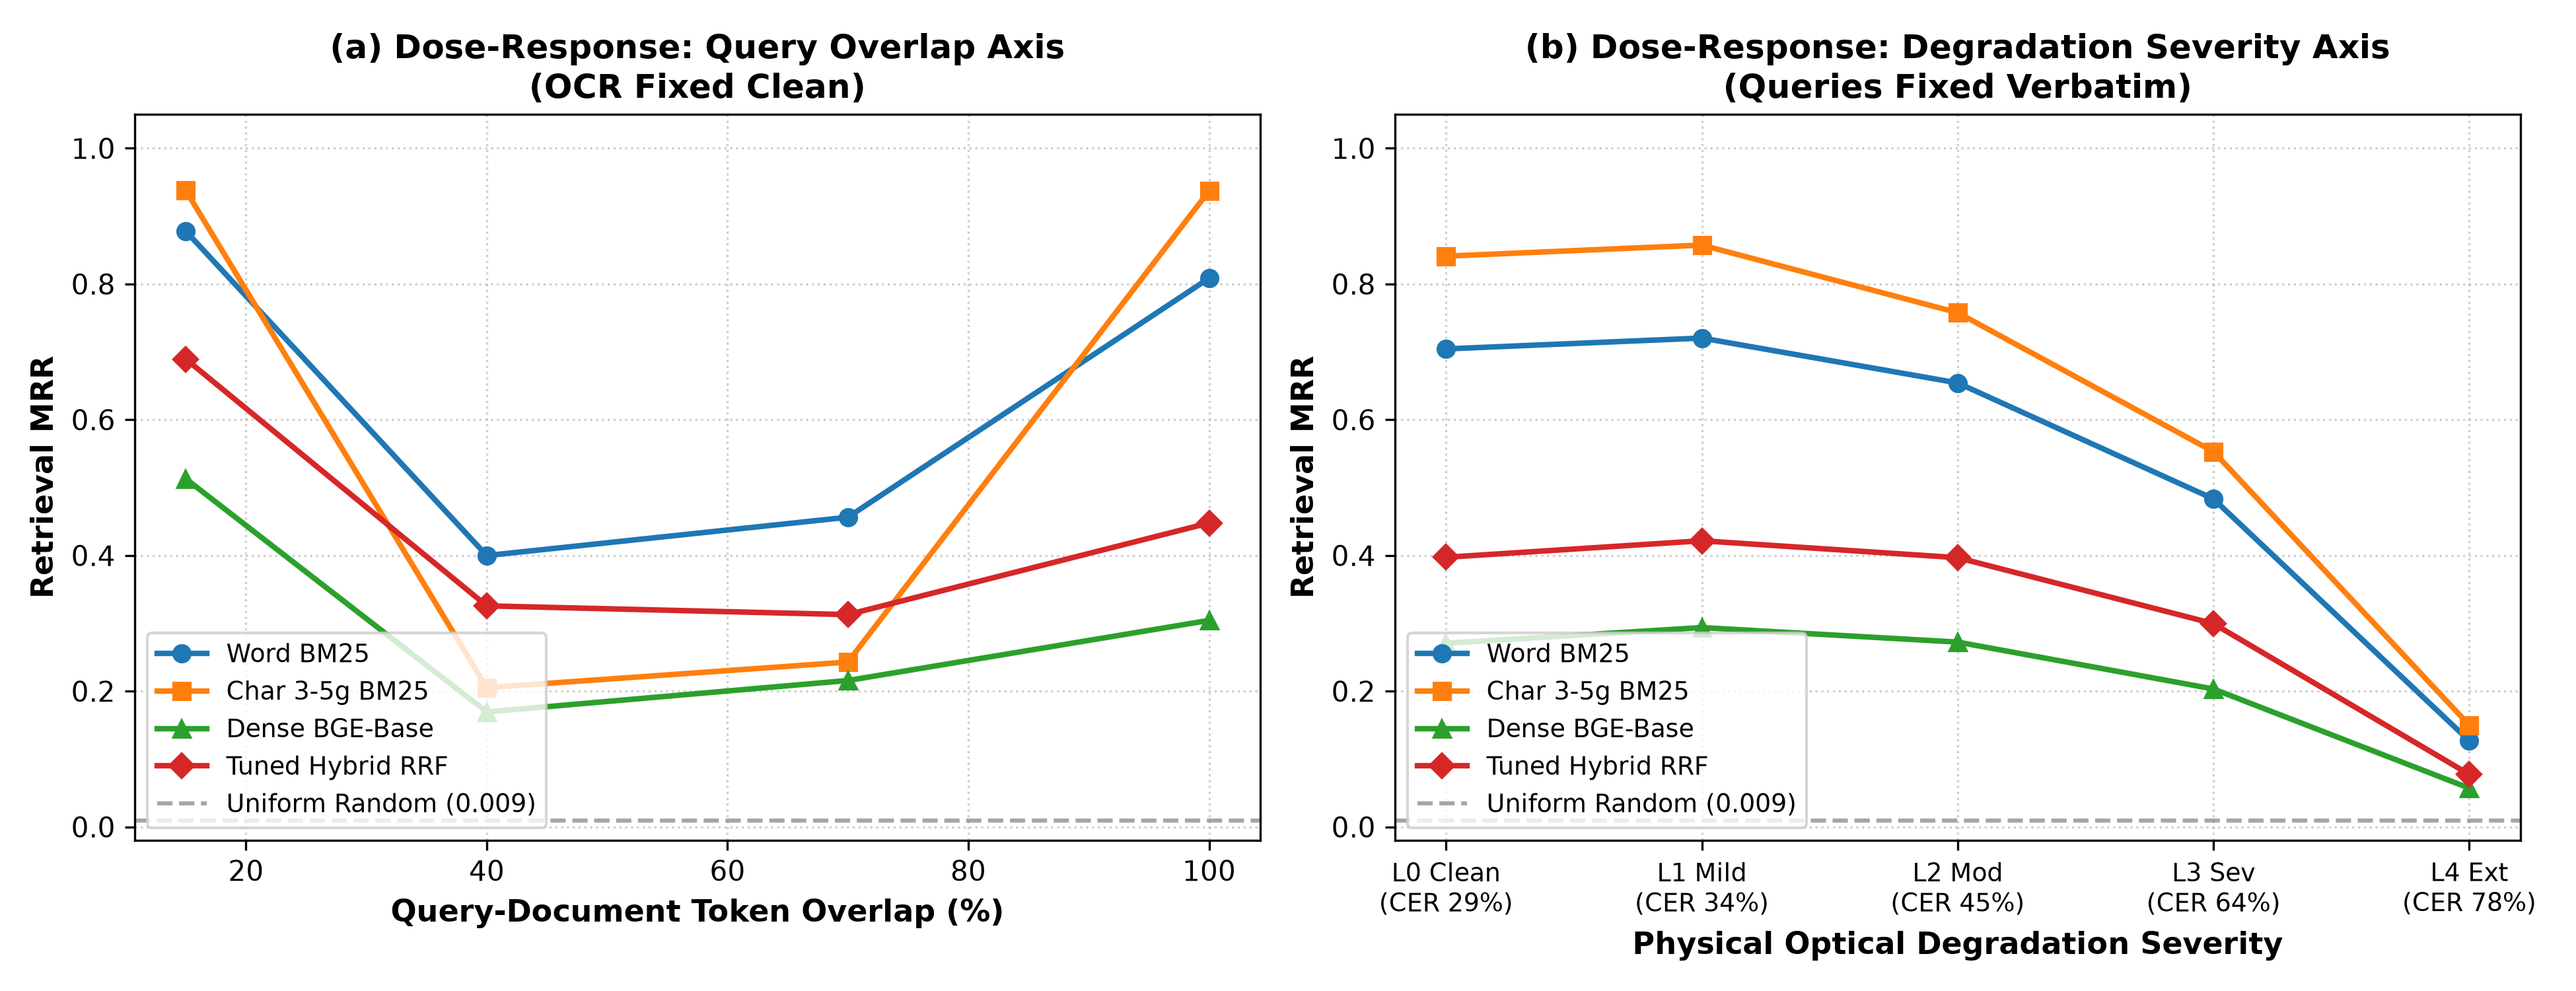
\includegraphics[width=0.80\columnwidth]{figures/fig_dose_response_dual_v6.png}
\caption{Dose-response retrieval surface across (a) query token overlap degradation from verbatim lookups to abstract questions, and (b) optical OCR degradation from pristine text to extreme Gaussian blur.}
\label{fig:dose_response_dual}
\end{figure}

\begin{enumerate}
    \setlength{\itemsep}{0.2pt plus 0.1pt}
    \setlength{\parskip}{0pt}
    \item \textbf{Verbatim Probes (Character Sub-Word Inverted Index Dominance):} Under verbatim lookups, character 3--5gram BM25 consistently outperforms word-level BM25 across all optical OCR conditions (Apple Clean: 0.9436 vs.\ 0.8371, diff $+0.1065$, $p < 10^{-4}$; Apple Degraded: 0.8248 vs.\ 0.6972, diff $+0.1276$, $p < 10^{-4}$; Tesseract Clean: 0.8412 vs.\ 0.7364, diff $+0.1048$, $p < 10^{-4}$; and 20\% synthetic noise: 0.7252 vs.\ 0.3961, diff $+0.3291$, $p < 10^{-4}$). Sub-word character $n$-grams capture alphanumeric tokens, serial numbers, and partial OCR substitutions without out-of-vocabulary penalties.
    \item \textbf{Light Paraphrase (Reversal of Dominance):} Introducing mild semantic paraphrasing collapses clean word BM25 from 0.8371 to 0.4334 (a 48\% relative drop) and character BM25 to 0.2427. In this regime, word BM25 outperforms character BM25 (diff $-0.1907$, $p < 10^{-4}$), and Dev-Tuned Hybrid achieves MRR = \textbf{0.4335} (clean OCR) and \textbf{0.1445} (20\% noise).
    \item \textbf{Answerable Factual Questions:} Evaluating natural answerable questions (forcing semantic abstraction while preserving topical anchors), character 3--5gram BM25 achieves MRR = \textbf{0.9471} on clean OCR and \textbf{0.8116} on degraded blur OCR, while word BM25 achieves 0.9014 and 0.7328. Tuned hybrid retrieval achieves 0.7705 on clean OCR and 0.5346 on degraded OCR, while dense BGE-base achieves 0.5128 and MiniLM achieves 0.2837. Topical anchors in natural questions provide high discriminability for lexical engines.
\end{enumerate}

To evaluate whether proxy corruption or semantic query mismatch is the dominant bottleneck in text-proxy RAG, we conducted paired permutation tests ($N_{\text{perm}}=100{,}000$). In Table~\ref{tab:regime_grid_v3}, moving from verbatim lookups to light paraphrasing on Apple Vision collapses Word BM25 by $\Delta = 0.4037$ MRR (0.8371 to 0.4334), exceeding optical blur degradation ($\Delta = 0.1399$, 0.8371 to 0.6972, $p < 10^{-5}$). Within Table~\ref{tab:engine_replication_v3} (receipt-only pool), Apple Vision drops 0.4321 MRR (0.8324 to 0.4003), while Tesseract drops 0.3400 under paraphrasing (0.7364 to 0.3964) and 0.3916 under optical blur (0.7364 to 0.3448). As visualized in Fig.~\ref{fig:mrr_regime_systems} and Fig.~\ref{fig:dose_response_dual}, semantic paraphrase mismatch dominates mild OCR noise, but severe optical blur induces comparable collapse.

\subsection{Micro-Mechanisms of Dense Collapse and Query Formulation Controls}
\label{sec:mechanism_analysis}

\begin{figure*}[t]
\centering
\begin{subfigure}[b]{0.30\textwidth}
    \centering
    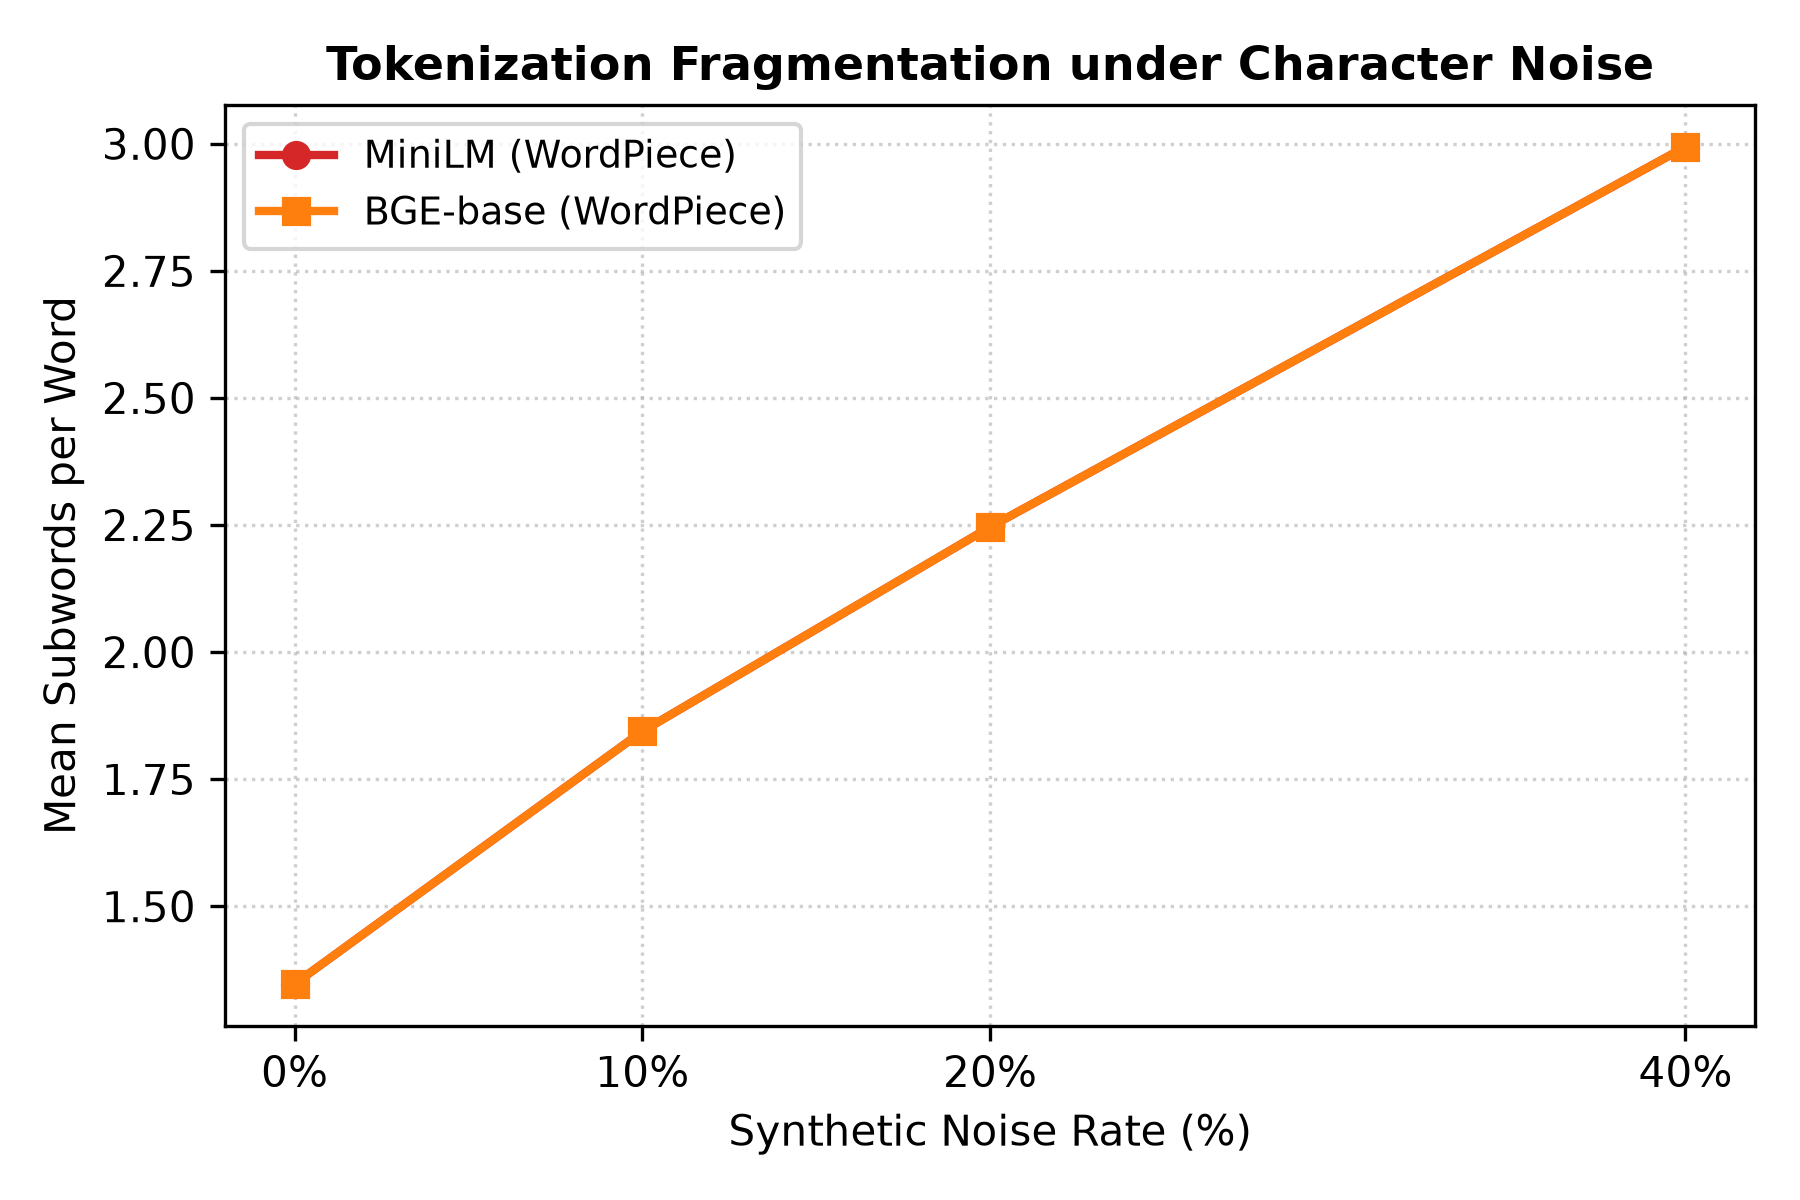
\includegraphics[width=\textwidth]{figures/fig_tokenization_fragmentation.png}
    \caption{Subword Fragmentation.}
    \label{fig:tokenization_fragmentation}
\end{subfigure}
\hfill
\begin{subfigure}[b]{0.30\textwidth}
    \centering
    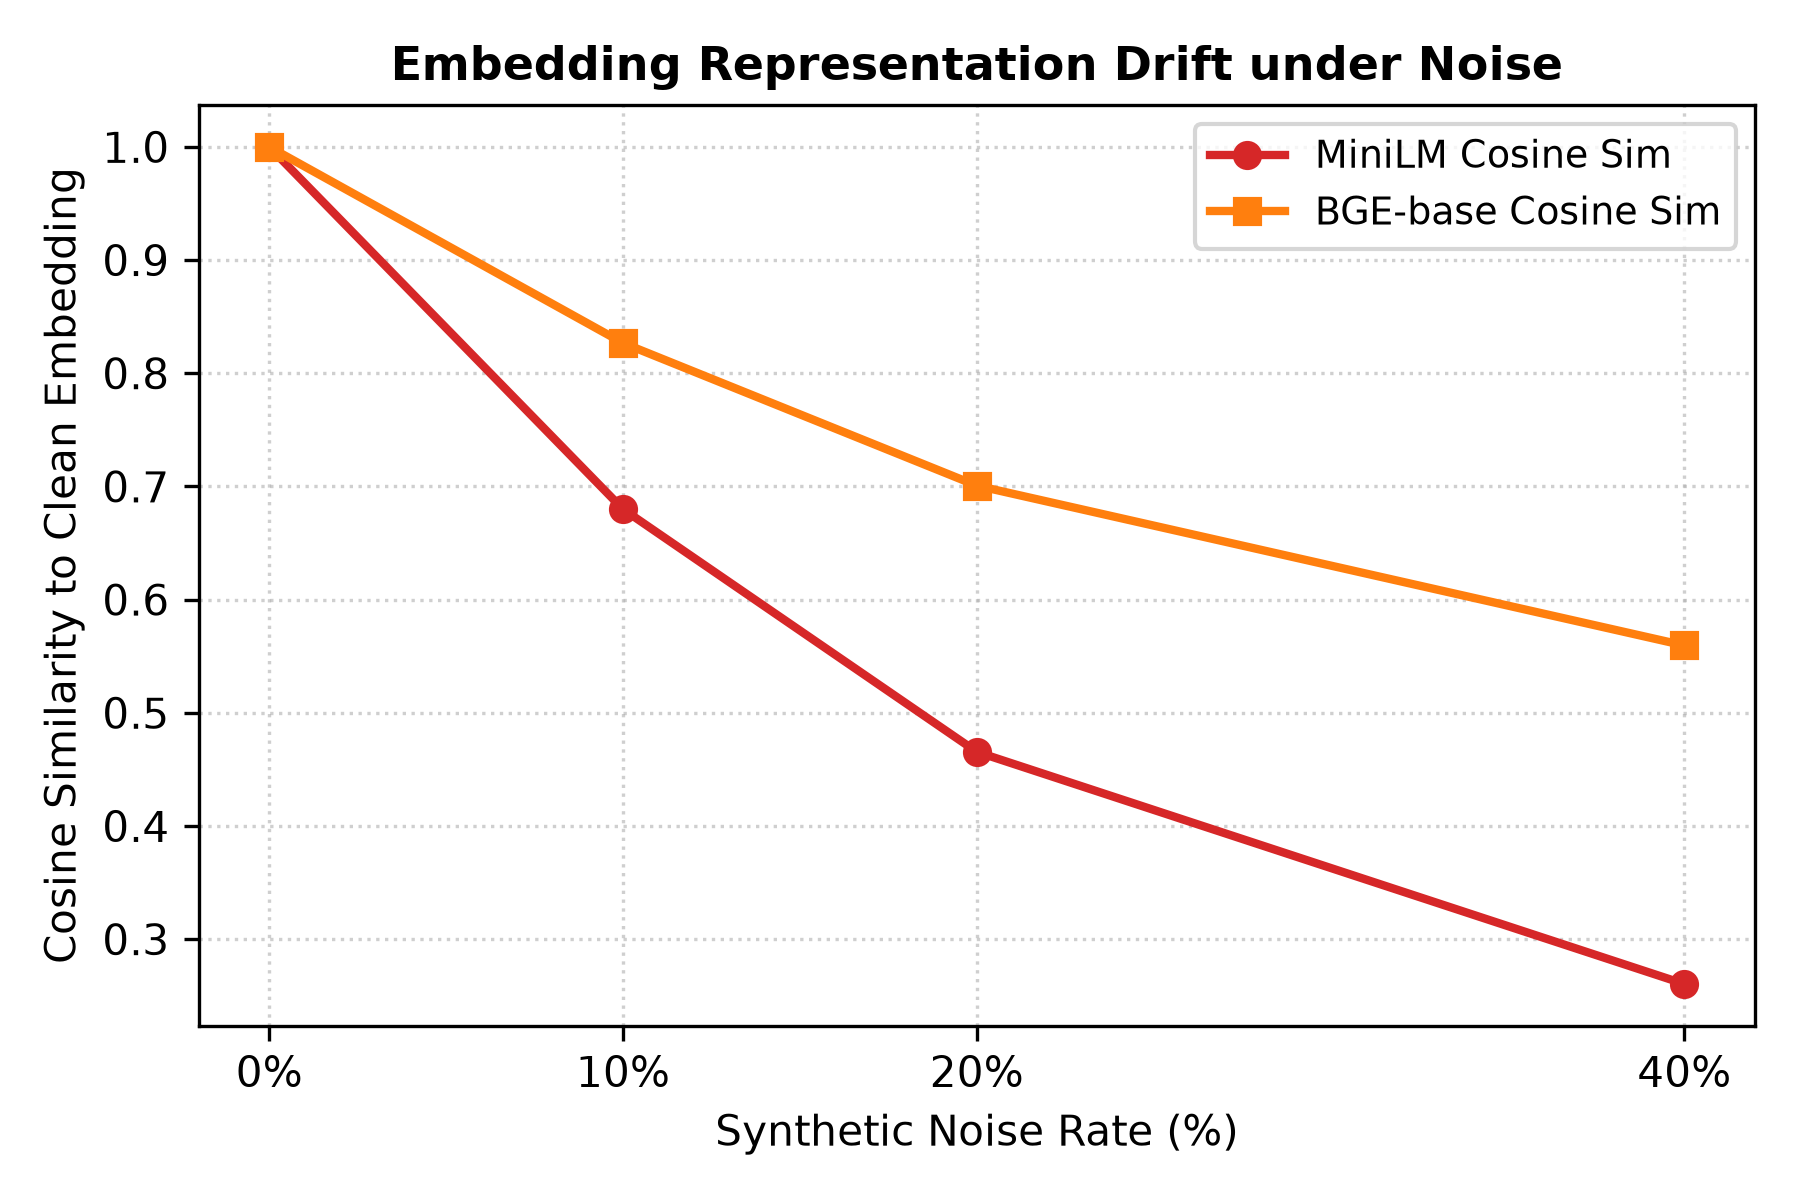
\includegraphics[width=\textwidth]{figures/fig_embedding_drift.png}
    \caption{Embedding Cosine Drift.}
    \label{fig:embedding_drift}
\end{subfigure}
\hfill
\begin{subfigure}[b]{0.30\textwidth}
    \centering
    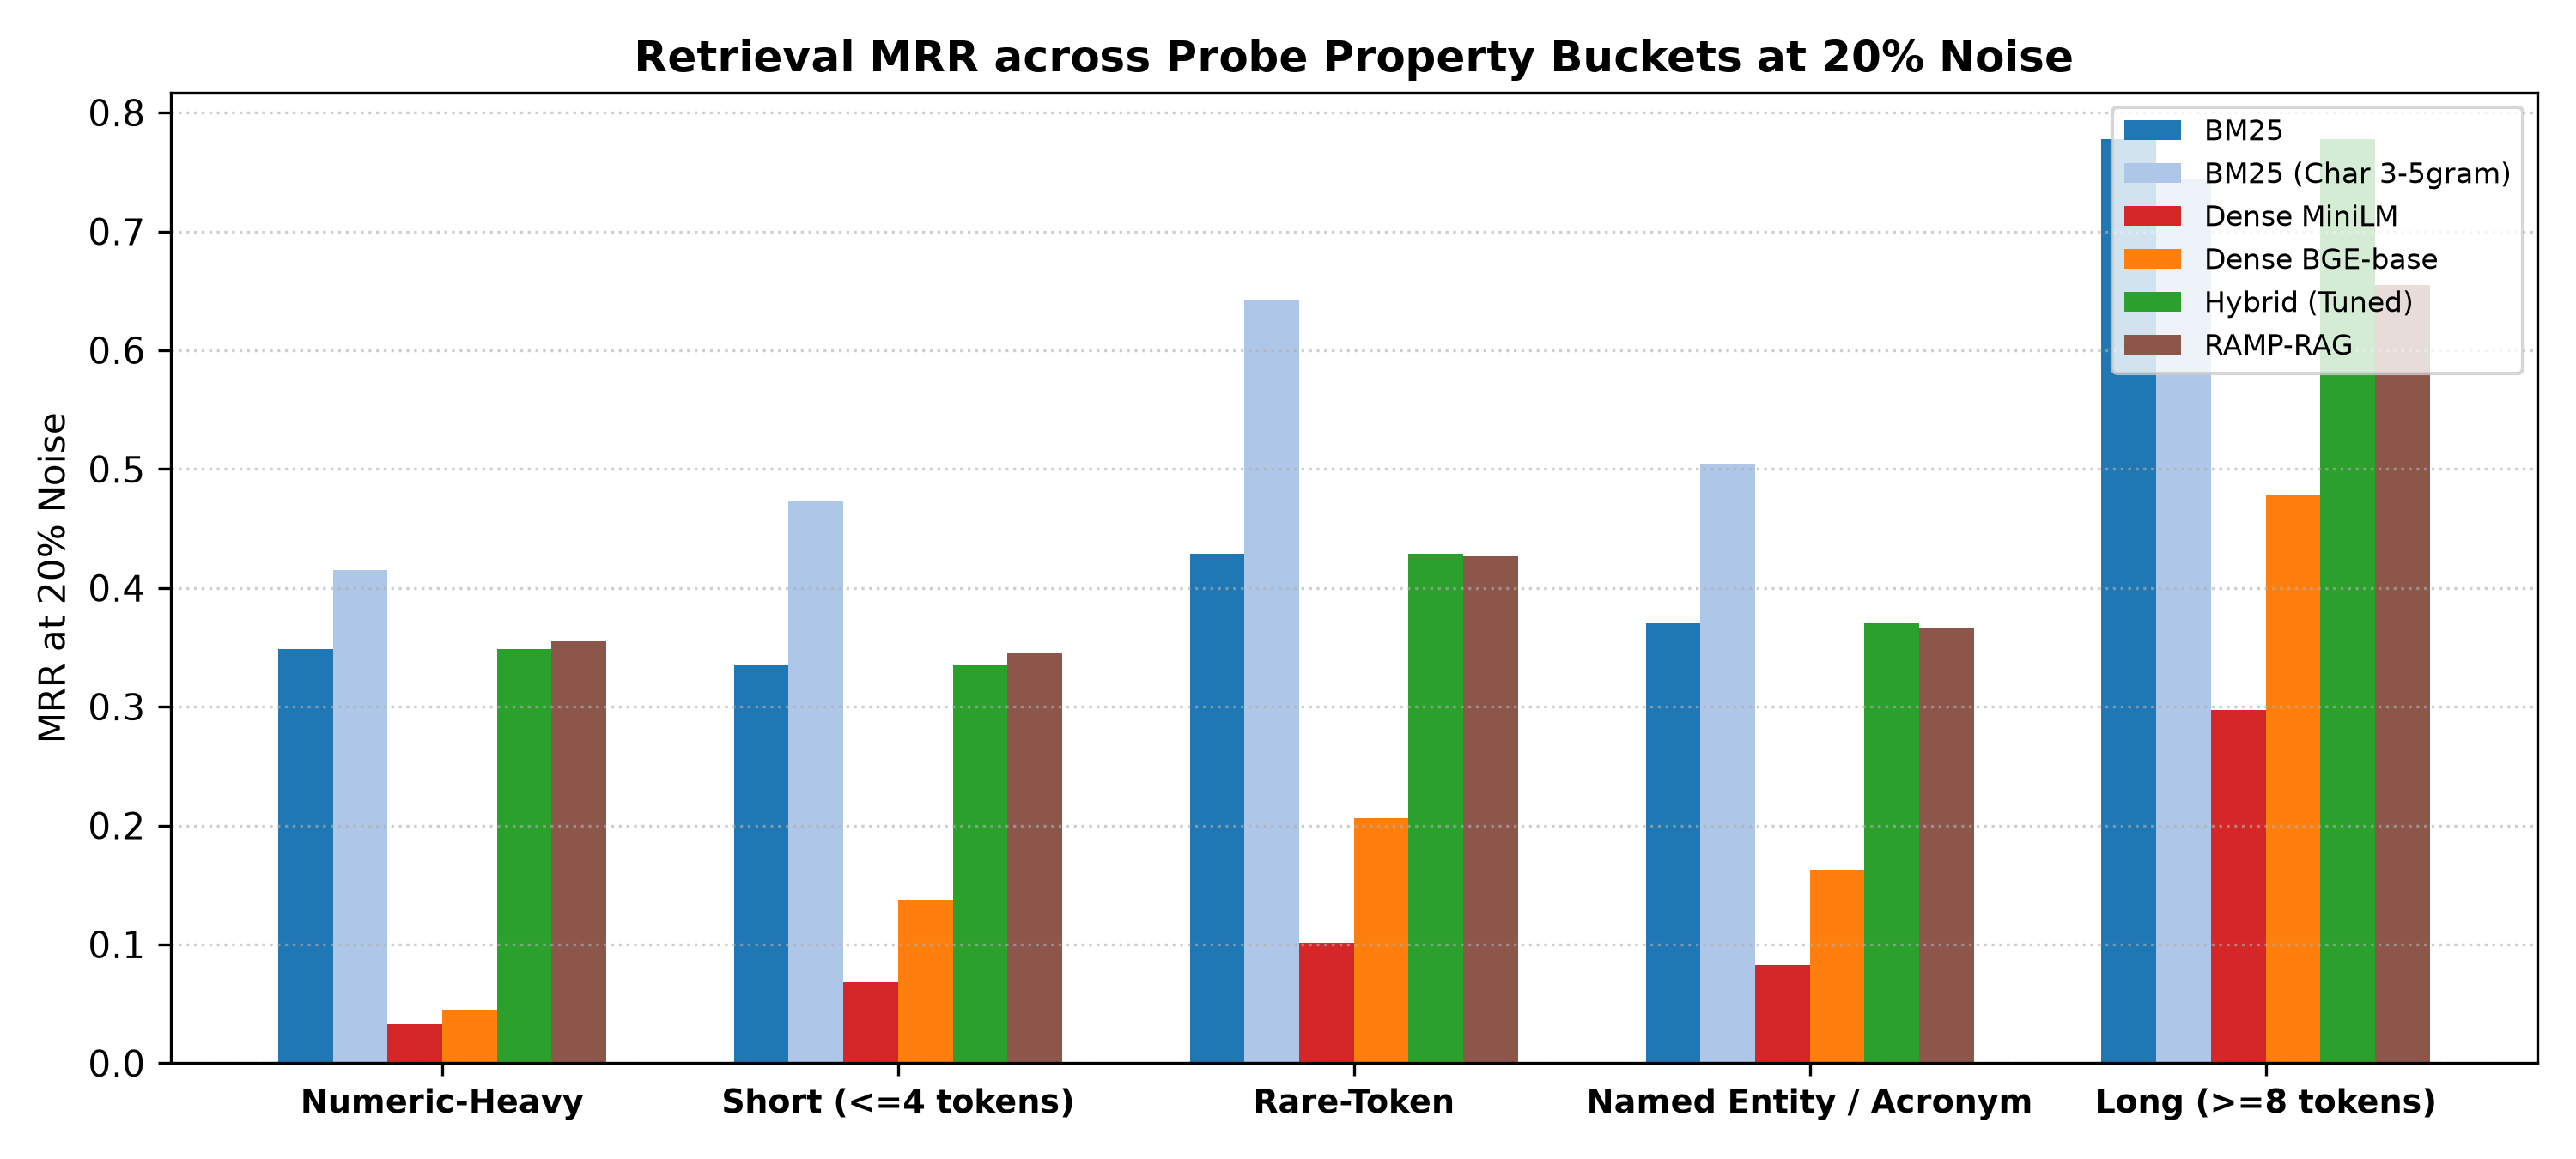
\includegraphics[width=\textwidth]{figures/fig_error_attribution.png}
    \caption{Probe Property Error Attribution.}
    \label{fig:error_attribution}
\end{subfigure}
\caption{Micro-mechanism of dense proxy collapse: (a) WordPiece tokenization fragmentation across character noise rates, (b) cosine embedding drift relative to clean representations, and (c) retrieval MRR across 5 diagnostic probe property buckets under 20\% proxy noise.}
\label{fig:mechanism_plots}
\end{figure*}

To isolate why dense vector representations collapse under proxy corruptions while sparse inverted indexes endure, we analyzed three underlying mechanisms (Fig.~\ref{fig:mechanism_plots}):
\begin{enumerate}
    \setlength{\itemsep}{0.2pt plus 0.1pt}
    \setlength{\parskip}{0pt}
    \item \textbf{WordPiece Tokenization Fragmentation:} As character corruption increases from 0\% to 40\%, WordPiece tokenization fragments words into multiple subwords. Mean subwords per word escalates from 1.347 (clean) to 1.774 (10\% noise), 2.246 (20\% noise), and \textbf{2.994} (40\% noise, a \textbf{+122.3\% increase}).
    \item \textbf{Catastrophic Embedding Drift:} Subword fragmentation shifts contextual attention weights, driving acute embedding drift. Relative to uncorrupted text, \texttt{all-MiniLM-L6-v2} mean cosine similarity collapses from 1.000 to 0.7301 (10\% noise), \textbf{0.4655} (20\% noise), and \textbf{0.2604} (40\% noise). \texttt{BAAI/bge-base-en-v1.5} displays greater structural resistance (cosine similarity 0.7007 at 20\% noise, 0.5595 at 40\%), explaining its superior noise resilience in Table~\ref{tab:regime_grid_v3}.
    \item \textbf{Diagnostic Error Attribution across Probe Properties:} Stratifying test probes into five property buckets under 20\% noise exposes distinct vulnerability profiles. Dense bi-encoders collapse on \emph{Numeric-Heavy} probes (MiniLM MRR = 0.033, BGE = 0.081) and \emph{Short} entity probes (MiniLM MRR = 0.068, BGE = 0.135). Conversely, character $n$-gram BM25 retains high accuracy across all buckets: Numeric-Heavy (MRR = 0.415), Short entities (0.473), Rare Tokens (0.643), and Named Entities (0.504).
\end{enumerate}

To verify whether dense degradation is an artifact of sequence length truncation, we evaluated token length distributions across all 626 SROIE receipts. While only 4 receipts (0.64\%) exceed 512 tokens, 209 of 626 receipts (33.39\%) exceed 256 WordPiece tokens. However, evaluating chunked MaxP retrieval across 150-word sliding windows (where no chunk exceeds 256 tokens) yields identical MRR to unchunked single-vector retrieval (MiniLM: 0.2030 chunked vs.\ 0.2056 unchunked; BGE-base: 0.3028 chunked vs.\ 0.3022 unchunked), demonstrating that sequence truncation is not the primary cause of dense collapse.

Crucially, as documented in Table~\ref{tab:dense_formulation_v6}, dense bi-encoder collapse on pristine ground truth text ($0\%$ noise) is strongly associated with query formulation mismatch. Short isolated verbatim snippets trigger severe representation disconnect (MiniLM MRR = 0.1919, BGE-Base MRR = 0.3256). Length-padding or wrapping snippets into sentential contexts does not alleviate the deficit. However, co-specifying multiple anchor entities (Keyword-Matched Probes) improves BGE-Base MRR to 0.5500 (Hit@10 78.43\%), and formulating queries as natural answerable questions improves BGE-Base MRR to 0.5263 (Hit@10 79.74\%) on the identical uncorrupted document text. Dense bi-encoders are trained on natural language question-passage pairs; when queries mirror real-world user questions rather than isolated OCR substrings, dense retrieval recovers substantial capacity.

Furthermore, to test the causal impact of tokenization fragmentation versus query formulation, we evaluated a vocabulary projection intervention against the clean Dev lexicon under 20\% character noise. Reconstructing broken word tokens restored 65.3\% of the induced WordPiece subword fragmentation and lifted cosine similarity by $+0.1530$ (from 0.6826 to 0.8356, recovering 48.2\% of embedding drift). In end-to-end retrieval, this intervention improves MiniLM MRR from 0.0570 to 0.1004 (+0.0434 retrieval recovery), while remaining bounded below clean baseline performance (0.2117 MRR). This vocabulary projection provides direct causal evidence that tokenization fragmentation contributes causally to noise-induced degradation, whereas the link between query formulation and clean-text retrieval remains an observational association.

\begin{table}[t]
\centering\small
\caption{Dense Bi-Encoder Sensitivity to Query Formulation on Clean Ground-Truth Receipt Text ($0\%$ noise, Test $N=306$).}\label{tab:dense_formulation_v6}
\resizebox{\columnwidth}{!}{%
\begin{tabular}{lcccc}
\toprule
Query Formulation & MiniLM MRR & MiniLM Hit@10 & BGE-Base MRR & BGE-Base Hit@10 \\
\midrule
1. Short Verbatim Snippets & 0.1919 & 0.2778 & 0.3256 & 0.3824 \\
2. Length-Padded Spans & 0.1949 & 0.2484 & 0.2571 & 0.3366 \\
3. Full Sentential Context Queries & 0.1670 & 0.2320 & 0.2740 & 0.3399 \\
4. Keyword-Matched Multi-Entity & 0.3840 & 0.5817 & 0.5500 & 0.7843 \\
5. Natural Answerable Questions & 0.3669 & 0.5686 & 0.5263 & 0.7974 \\
\bottomrule
\end{tabular}}
\vspace{-2mm}
\end{table}

\subsection{Production Cascades and Risk-Controlled Escalation}
\label{sec:ablation_and_cascade}

Table~\ref{tab:ablation_v3} presents the component ablation isolating each architectural module across Clean, 20\% Synthetic Noise, Real Apple Vision OCR, and Real Degraded OCR ($N=306$ held-out probes). In Table~\ref{tab:ablation_v3}, the Fixed-weight Hybrid baseline evaluates candidate depth $K_1=10$ with equal-weight dense interpolation ($\alpha=0.5$), where dense bi-encoder deficit pulls Real-OCR MRR (0.8121) slightly below standalone BM25 (0.8371). Passing top-$K_1$ candidates through cross-encoder rerankers elevates performance to 0.8426 (MiniLM) and 0.8555 (BGE-reranker). When evaluated under the production setting in Table~\ref{tab:practical_stack} with candidate depth $K_1=20$ directly over first-stage Word BM25 (0.8371), BGE-reranker-base reaches 0.8846 (+0.0475 gain, $p=0.0011$).

\begin{table*}[t]
\centering
\small
\caption{Architectural Component Ablation on Public Held-Out Test Split ($N=306$ Probes, 813 Distractor Pool, 95\% Cluster Bootstrap CIs). Asterisks ($^*$) denote statistically significant difference ($p_{\text{Holm}} < 0.05$) from the Fixed-weight Hybrid baseline (candidate depth $K_1=10$). In contrast, Table~\ref{tab:practical_stack} cascades top $K_1=20$ candidates directly over first-stage Word BM25 (0.8371), reaching 0.8846. Note: In Table~\ref{tab:ablation_v3}, the Fixed-weight Hybrid baseline evaluates candidate depth $K_1=10$ with equal-weight dense interpolation, where dense deficit pulls Real-OCR MRR (0.8121) slightly below standalone BM25 (0.8371).}
\label{tab:ablation_v3}
\resizebox{\textwidth}{!}{%
\begin{tabular}{lcccc}
\toprule
Configuration & Clean MRR [95\% CI] & Syn 20\% MRR [95\% CI] & Real-OCR MRR [95\% CI] & Real-Deg MRR [95\% CI] \\
\midrule
Fixed-weight Hybrid Baseline ($K_1=10$) & 0.8299 [0.791, 0.866] & 0.3694 [0.336, 0.402] & 0.8121 [0.770, 0.849] & 0.6684 [0.619, 0.715] \\
+ Clean Stream                  & 0.8299 [0.791, 0.866] & 0.3694 [0.336, 0.402] & 0.8121 [0.770, 0.849] & 0.6684 [0.619, 0.715] \\
BM25 + Clean Stream             & 0.8317 [0.793, 0.868] & 0.3694 [0.336, 0.402] & 0.8069 [0.766, 0.845] & 0.6702 [0.621, 0.716] \\
Dense + Clean Stream            & 0.2144$^*$ [0.175, 0.256] & 0.0747$^*$ [0.057, 0.095] & 0.2072$^*$ [0.168, 0.248] & 0.1821$^*$ [0.143, 0.222] \\
+ Learned Router (H2)           & 0.8309 [0.793, 0.867] & 0.3765$^*$ [0.343, 0.409] & 0.8121 [0.770, 0.849] & 0.6667 [0.617, 0.712] \\
+ Heuristic Reliability Weighting& 0.8318 [0.794, 0.867] & 0.3574 [0.326, 0.390] & 0.8058 [0.765, 0.843] & 0.6368$^*$ [0.587, 0.684] \\
+ Cascade (MiniLM, $K_1=10$)    & 0.8709$^*$ [0.836, 0.903] & 0.4033$^*$ [0.369, 0.436] & 0.8426$^*$ [0.801, 0.878] & 0.6879 [0.638, 0.735] \\
+ Cascade (BGE-reranker, $K_1=10$)& 0.8821$^*$ [0.848, 0.913] & 0.4154$^*$ [0.382, 0.448] & 0.8555$^*$ [0.816, 0.890] & 0.6969 [0.645, 0.745] \\
Full System (MiniLM)            & 0.8771$^*$ [0.843, 0.909] & 0.4132$^*$ [0.378, 0.450] & 0.8451$^*$ [0.805, 0.880] & 0.6786 [0.629, 0.727] \\
Full System (BGE-reranker)      & 0.8873$^*$ [0.854, 0.917] & 0.4200$^*$ [0.384, 0.456] & 0.8554$^*$ [0.816, 0.891] & 0.6755 [0.625, 0.724] \\
\midrule
BM25 Alone                      & 0.8317 [0.793, 0.868] & 0.3694 [0.336, 0.402] & 0.8371 [0.798, 0.871] & 0.6684 [0.619, 0.714] \\
All-Stream RRF (Strawman)       & 0.3227$^*$ [0.283, 0.365] & 0.1827$^*$ [0.156, 0.212] & 0.3079$^*$ [0.269, 0.350] & 0.2791$^*$ [0.239, 0.322] \\
\bottomrule
\end{tabular}}
\end{table*}

However, evaluating two-stage cascades over first-stage Character 3--5gram BM25 reveals an architectural ceiling: standalone Char-BM25 achieves MRR = \textbf{0.9437}, and applying MiniLM or BGE cross-encoders on top-20 candidates reduces MRR to 0.9175 and 0.9141 (lifts of $-0.0262$ and $-0.0296$, Table~\ref{tab:practical_stack}). Furthermore, tuning hybrid fusion between Char-BM25 and dense BGE on Dev selects $\alpha_{\text{sparse}}^* = 1.00$ ($\alpha_{\text{dense}}^* = 0.00$, 0.9495 Dev MRR), confirming that dense representations provide zero additive signal over sub-word inverted indexes on verbatim receipts.

\begin{table}[htbp]
\centering
\small
\caption{Production Cross-Encoder Reranker Cascade Ablation (Held-Out Test Split, $N=306$ Probes, Clean Real-OCR; Candidate Depth $K_1=20$).}
\label{tab:practical_stack}
\resizebox{\columnwidth}{!}{%
\begin{tabular}{lcccc}
\toprule
Two-Stage Retrieval Pipeline & Clean MRR & Hit@10 & Latency (ms) & MRR Lift ($p$-value) \\
\midrule
Word BM25 (First-Stage Alone)    & 0.8371 & 0.9444 & 0.1 & +0.0000 ($p=1.0$) \\
BM25 + MiniLM Cross-Encoder      & 0.8650 & 0.9608 & 18.4 & +0.0279 ($p=0.0092$) \\
BM25 + BGE-reranker-base         & 0.8846 & 0.9738 & 44.7 & +0.0475 ($p=0.0011$) \\
Tuned Hybrid + BGE-reranker      & 0.8872 & 0.9772 & 52.8 & +0.0501 ($p=0.0009$) \\
\midrule
Char 3--5g BM25 Standalone       & \textbf{0.9437} & \textbf{0.9837} & 0.96 & Baseline (Sparse) \\
Char BM25 + MiniLM Reranker      & 0.9175 & 0.9706 & 18.5 & -0.0262 (Hurts) \\
Char BM25 + BGE Reranker         & 0.9141 & 0.9771 & 44.7 & -0.0296 (Hurts) \\
Tuned Char-BM25 + BGE ($\alpha_{\text{sparse}}=1.00$) & \textbf{0.9437} & \textbf{0.9837} & 12.6 & +0.0000 ($p=1.0$) \\
\bottomrule
\end{tabular}}
\vspace{-2mm}
\end{table}

\textbf{Finite-Sample Conformal Cascade Risk Evaluation:}
To evaluate distribution-free marginal risk control for candidate escalation, we evaluated split conformal calibration across 200 random cluster-stratified 50/50 splits (seeds 1000--1199) on $N=2{,}754$ pooled query instances (Table~\ref{tab:conformal_cascade_v6}). The evaluation instances comprise three equal query slices ($3 \times 918$ instances): verbatim lookups, entity rewrites, and legacy token-stripped probes, evaluated across clean, 20\% synthetic noise, and real OCR document streams. When calibrated under marginal loss $L = \mathbf{1}[\text{not escalated} \land Y \ne 1]$ with finite-sample adjustment $(n\hat{R}+1)/(n+1) \le \alpha$ \cite{bates2021conformal, angelopoulos2021gentle}, the observed mean test miss risk is $0.0494$ at an escalation rate of $78.4\%$.

\begin{table}[t]
\centering\small
\caption{Conformal Cascade Calibration: Corrected Marginal Loss, High-Probability RCPS ($\delta=0.10$), and Equal-Escalation Baseline over 200 Cluster-Aware Splits ($N=2{,}754$ instances across verbatim, entity rewrites, and token-stripped probe slices; nominal target $\epsilon=0.05$).}\label{tab:conformal_cascade_v6}
\resizebox{\columnwidth}{!}{%
\begin{tabular}{lccccc}
\toprule
Risk Formulation & Mean $\tau^*$ & Mean Test Risk & Split Cov. ($\le 0.05$) & Mean Esc. Rate & Mean MRR \\
\midrule
Marginal Loss $L=\mathbf{1}[\text{not esc} \land \text{miss}]$ & 0.2369 & 0.0494 & 58.5\% & 78.4\% & 0.3577 \\
High-Probability RCPS ($\delta=0.10$) & 0.2520 & 0.0429 & \textbf{82.0\%} & 79.5\% & 0.3569 \\
Equal-Escalation Fixed Margin ($\tau=0.235$) & 0.2347 & 0.0488 & 57.0\% & 78.4\% & 0.3579 \\
Conditional Ratio $P(\text{miss} \mid \text{not esc})$ & 0.4071 & 0.0545 & 38.0\% & 90.2\% & 0.3524 \\
\bottomrule
\end{tabular}}
\vspace{-2mm}
\end{table}

\begin{figure}[t]
\centering
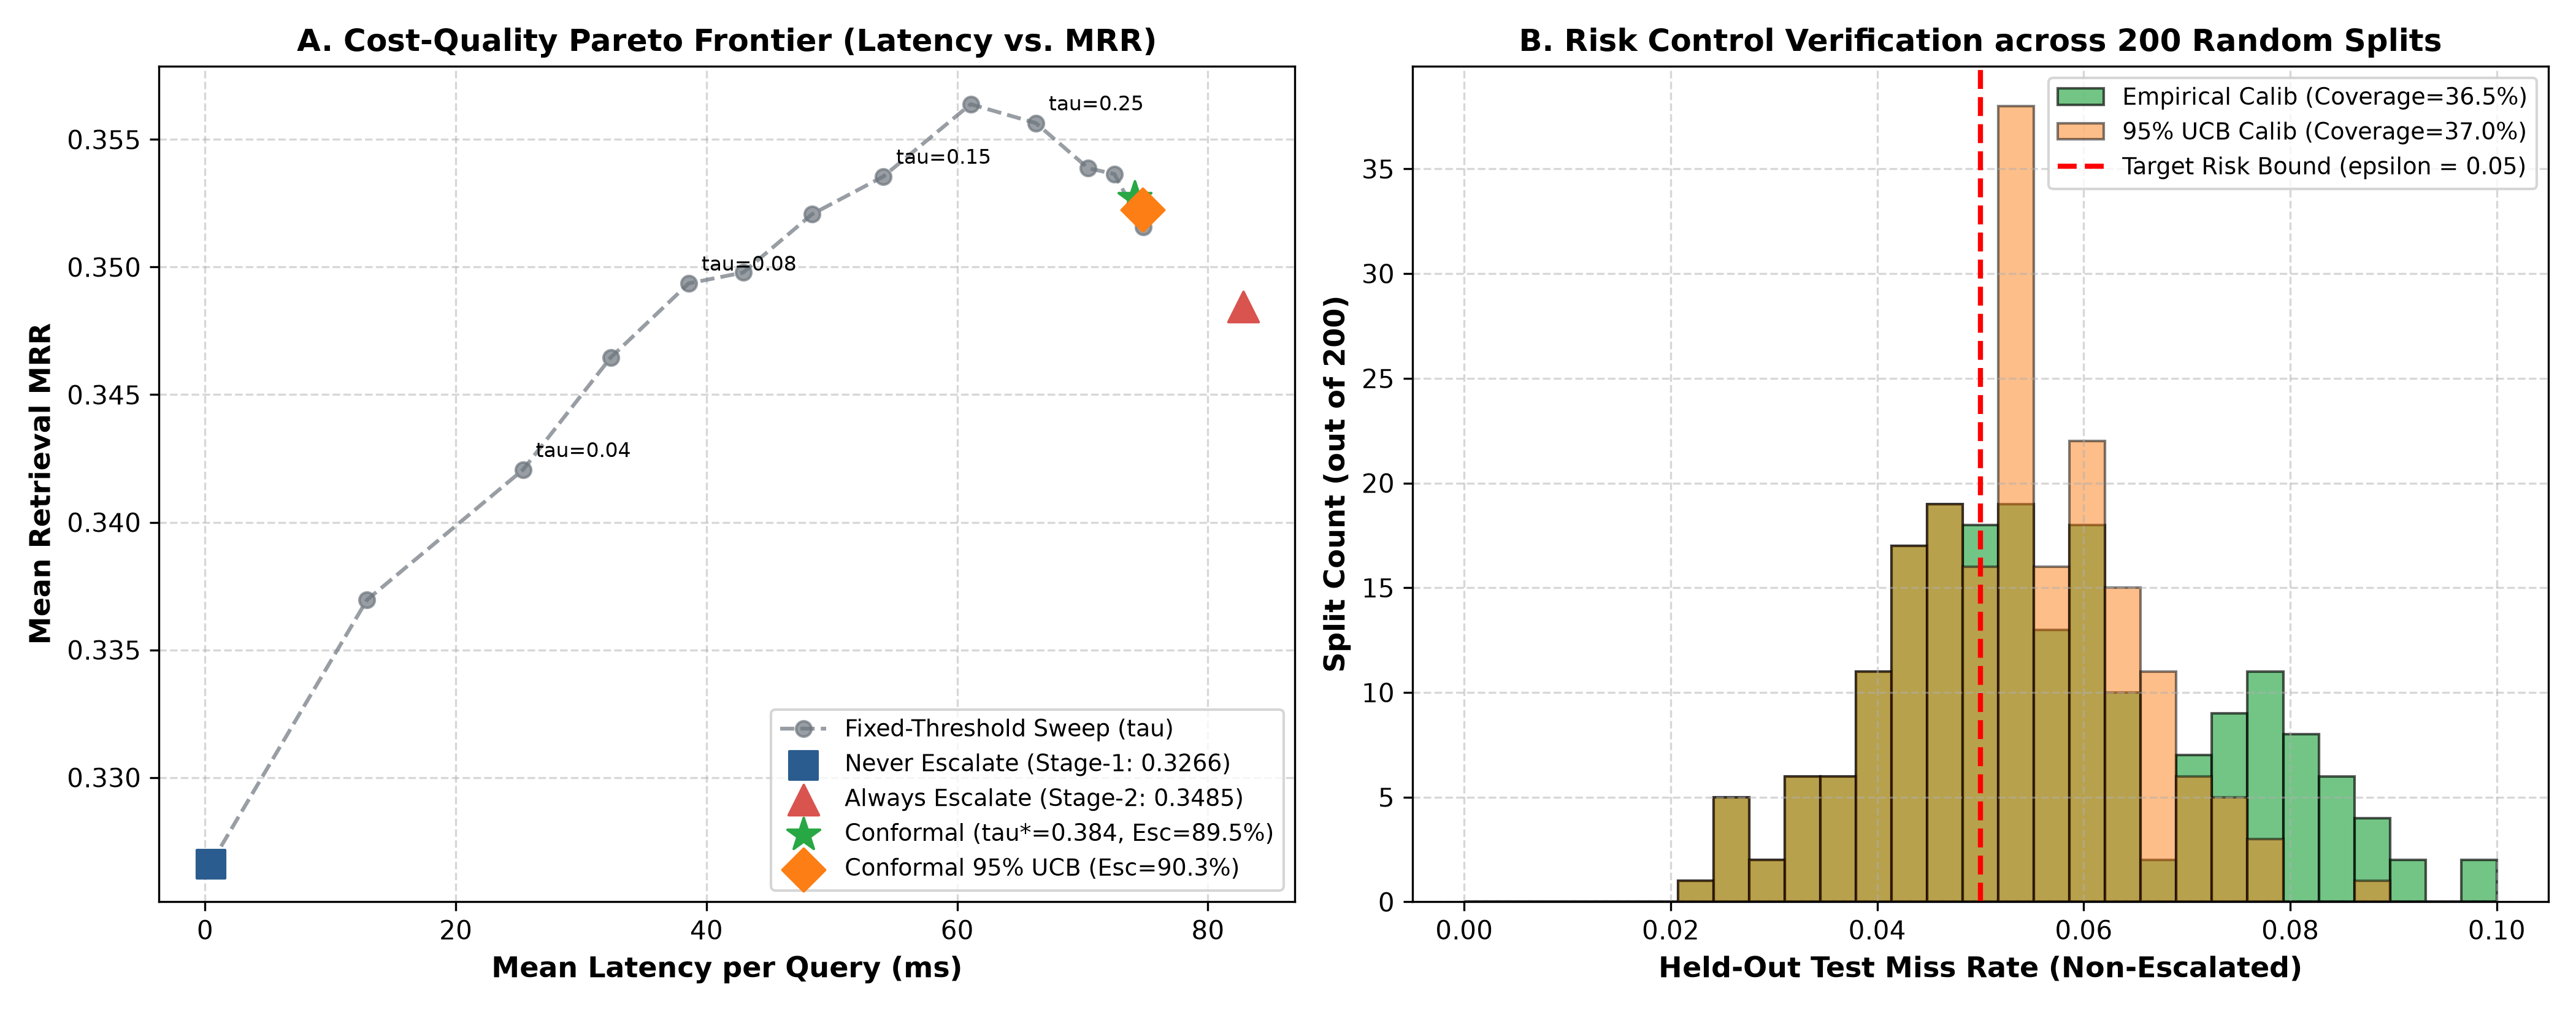
\includegraphics[width=0.80\columnwidth]{figures/fig_conformal_pareto.png}
\caption{Cost-Quality Pareto frontier and risk control histogram across 200 random splits under conformal cascade calibration.}
\label{fig:conformal_pareto}
\end{figure}

Because the 200 splits resample the same fixed pool of $N=2{,}754$ instances, the reported interval $[0.0480, 0.0502]$ describes only the sample mean across partitions of this pool, not a generalization CI for unseen queries or documents. The 10th-to-90th percentile range across splits is $[0.0355, 0.0654]$. Crucially, empirical split coverage (risk $\le 0.05$) is only 58.5\%, below nominal 95\% single-split coverage. Furthermore, a paired comparison against an equal-escalation fixed-margin baseline calibrated at the identical 78.4\% escalation rate ($\tau = 0.235$) reveals that fixed-margin escalation matches conformal calibration in realized retrieval accuracy (MRR 0.3579 vs.\ 0.3577, $p > 0.05$) and risk control (0.0488 vs.\ 0.0494; coverage 57.0\% vs.\ 58.5\%). Stratified by query type, entity rewrites experience risk 0.0627 ($>0.05$), demonstrating that marginal calibration does not guarantee conditional protection per query slice. Conformal calibration evaluates cross-encoders on 78.4\% of queries, which represents a 21.6\% escalation reduction strictly relative to an all-escalation baseline (Fig.~\ref{fig:conformal_pareto}).

\subsection{Regime B: Visual-Dominated Natural Image Search}
\label{sec:regime_b_visual}

To evaluate representation boundaries on non-document imagery, we benchmarked $N=1{,}000$ MS-COCO Karpathy-test images \cite{karpathy2015deep, lin2014coco} and held-out human descriptions (Table~\ref{tab:coco_benchmarks_v3}).

\begin{table}[htbp]
\centering
\small
\caption{Cross-modal text-to-image retrieval performance on $N=1{,}000$ MS-COCO Karpathy-test images. Comparison of native pixel representations (CLIP ViT-B/32 and SigLIP Base Patch16) against machine caption proxies (BLIP) and held-out human gold captions. Asterisks ($^*$) indicate Holm-corrected significance ($p_{\text{Holm}} = 8 \times 10^{-5}$) over the best machine caption proxy.}
\label{tab:coco_benchmarks_v3}
\resizebox{\columnwidth}{!}{%
\begin{tabular}{lcccc}
\toprule
Method & Hit@1 & Hit@5 & Hit@10 [95\% CI] & MRR [95\% CI] \\
\midrule
\multicolumn{5}{l}{\textit{Machine Caption Proxy (BLIP)}} \\
BM25                          & 0.1220 & 0.2800 & 0.3840 [0.355, 0.415] & 0.2048 [0.186, 0.225] \\
Dense MiniLM (Best BLIP Proxy)& 0.2420 & 0.5160 & 0.6530 [0.624, 0.682] & 0.3728 [0.350, 0.397] \\
Dense BGE-base                & 0.2430 & 0.5050 & 0.6460 [0.618, 0.678] & 0.3695 [0.347, 0.393] \\
\midrule
\multicolumn{5}{l}{\textit{Human Gold Caption Proxy (Upper Bound)}} \\
BM25 (Gold Proxy)             & 0.3600 & 0.6250 & 0.7350 [0.708, 0.762] & 0.4852 [0.461, 0.510] \\
Dense MiniLM (Gold Proxy)     & 0.4550 & 0.7280 & 0.8380 [0.814, 0.860] & 0.5801 [0.555, 0.605] \\
Dense BGE-base (Gold Proxy)   & 0.4580 & 0.7370 & 0.8320 [0.809, 0.854] & 0.5835 [0.559, 0.608] \\
\midrule
\multicolumn{5}{l}{\textit{Native Pixel Representation}} \\
\textbf{CLIP ViT-B/32}        & \textbf{0.3390}$^*$ & \textbf{0.6180}$^*$ & \textbf{0.7570}$^*$ [0.729, 0.785] & \textbf{0.4709}$^*$ [0.446, 0.497] \\
\textbf{SigLIP Base Patch16}  & \textbf{0.4800}$^*$ & \textbf{0.7680}$^*$ & \textbf{0.8670}$^*$ [0.845, 0.888] & \textbf{0.6071}$^*$ [0.584, 0.633] \\
\midrule
\multicolumn{5}{l}{\textit{Multi-Vector \& Hybrid Fusion}} \\
Hybrid (CLIP + BGE BLIP)      & 0.3880 & 0.6720 & 0.7870 [0.760, 0.811] & 0.5186 [0.494, 0.544] \\
Hybrid (SigLIP + BGE BLIP)    & 0.4570 & 0.7470 & 0.8360 [0.813, 0.858] & 0.5866 [0.563, 0.611] \\
All-Stream RRF (Strawman)     & 0.2690 & 0.5530 & 0.6890 [0.662, 0.718] & 0.4058 [0.382, 0.429] \\
\bottomrule
\end{tabular}}
\vspace{-2mm}
\end{table}

\begin{figure}[t]
\centering
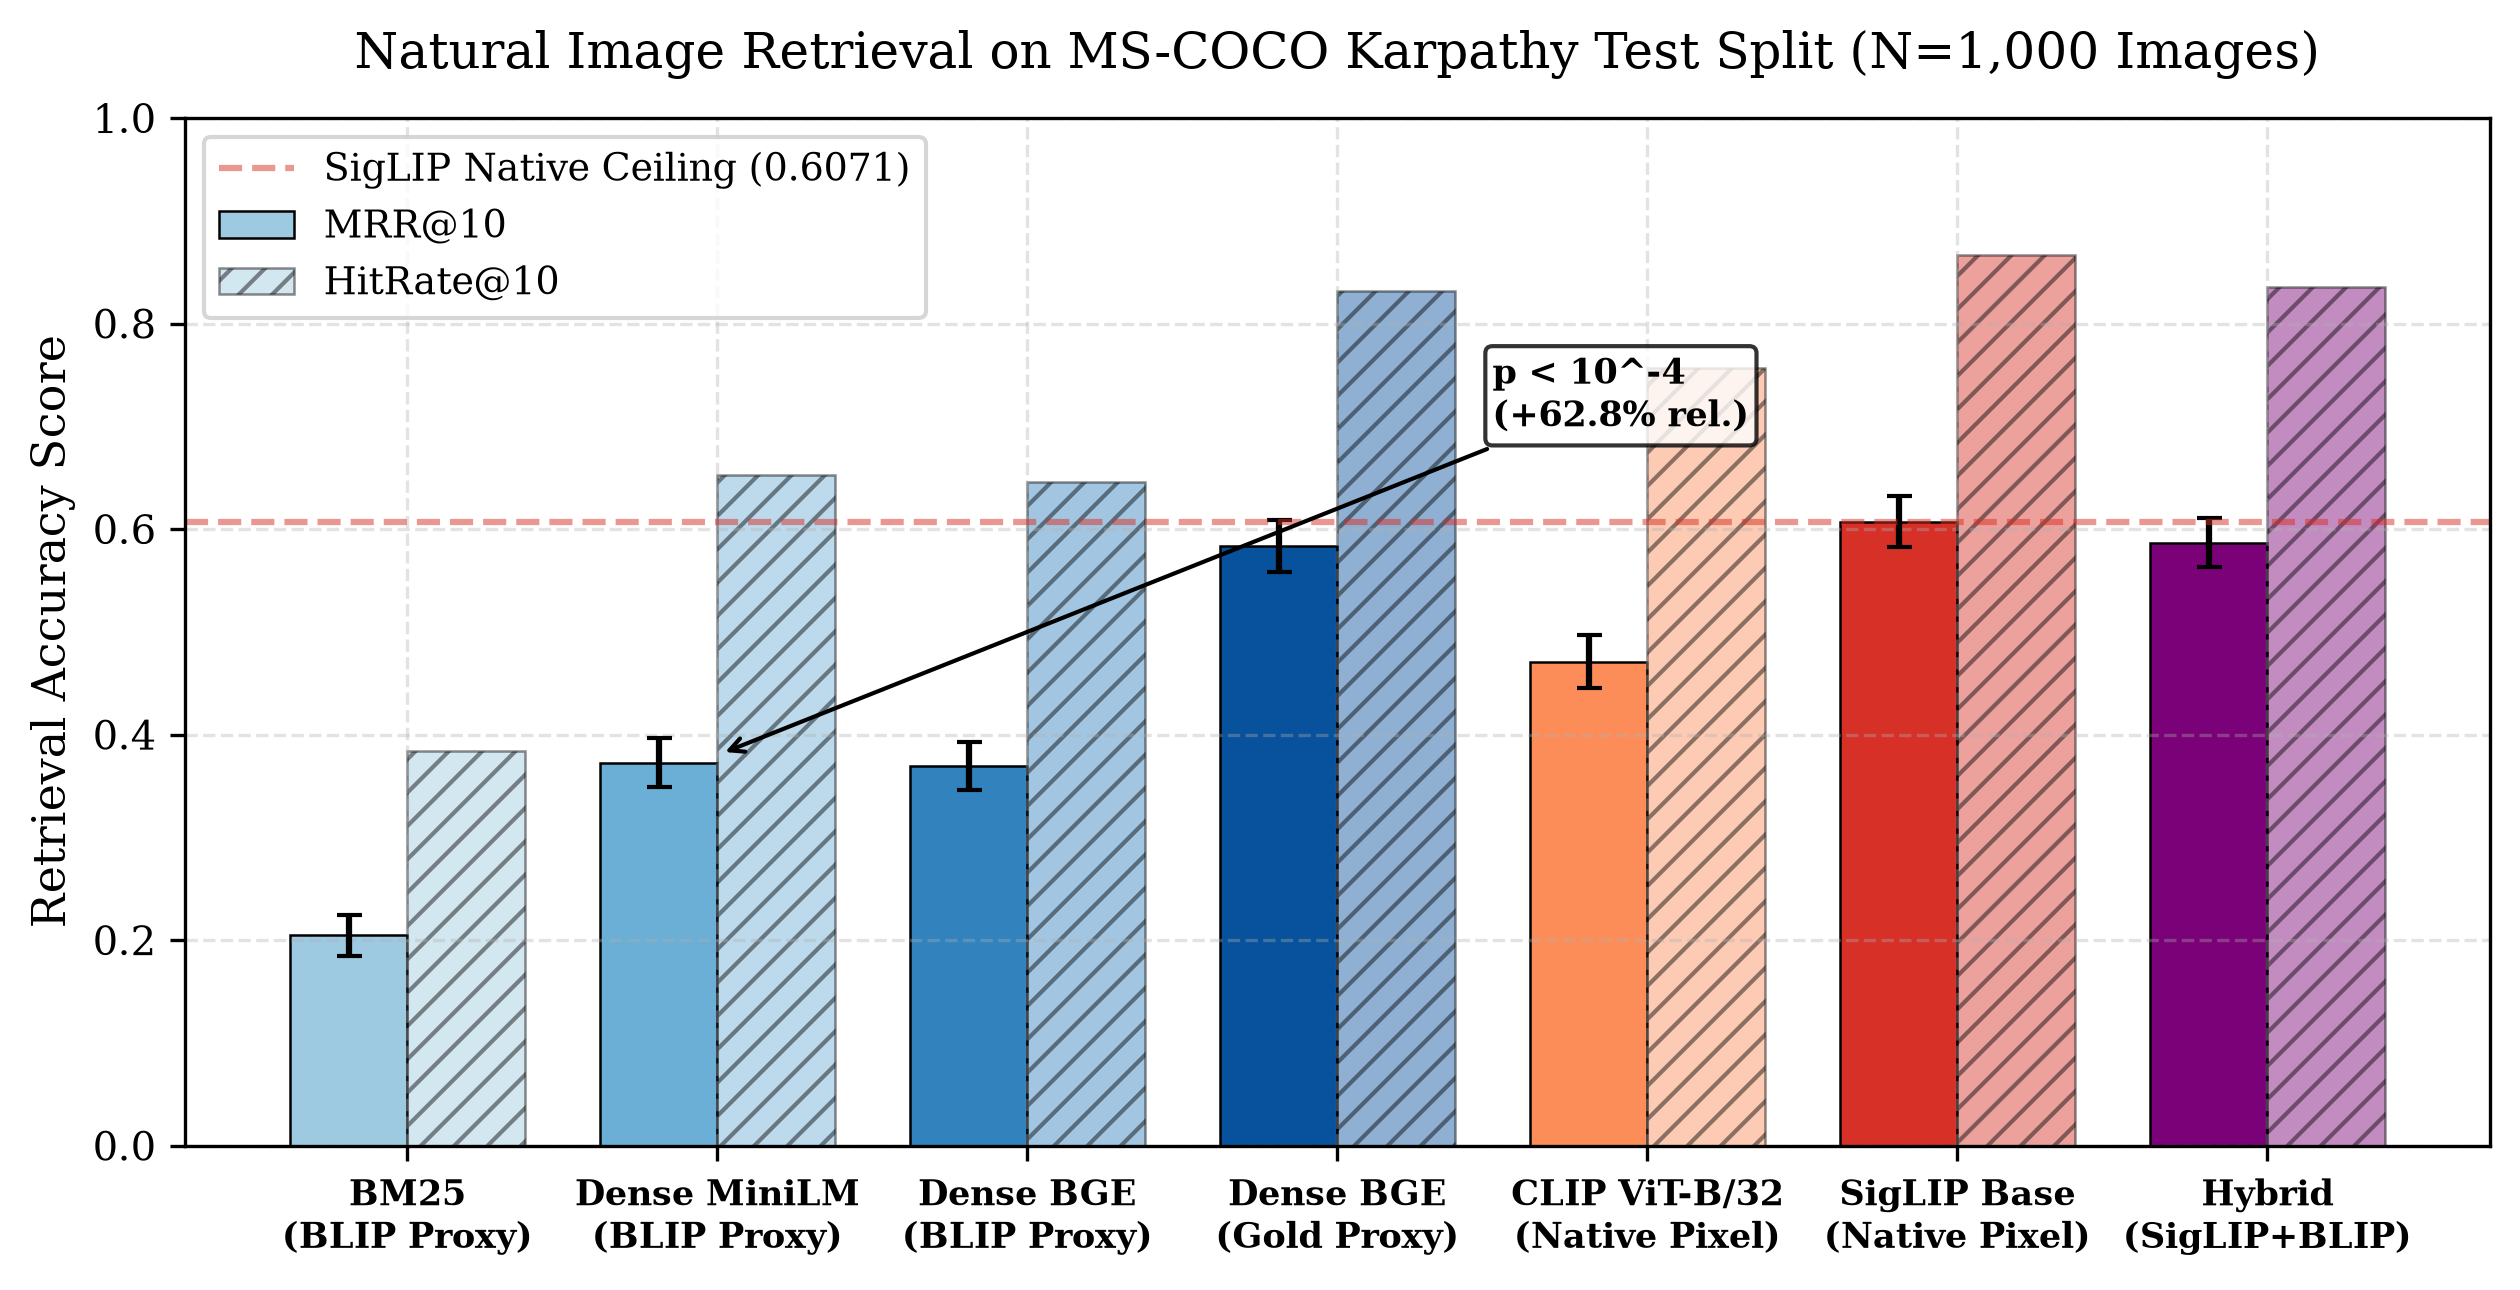
\includegraphics[width=0.80\columnwidth]{figures/fig_coco_native_vs_proxy.png}
\caption{Retrieval comparison on MS-COCO ($N=1{,}000$ images): native visual embeddings (SigLIP Base Patch16) significantly outperform machine-generated caption proxies ($p < 10^{-4}$), demonstrating that text proxies incur substantial information loss on natural imagery.}
\label{fig:coco_native_vs_proxy}
\end{figure}

Native visual representations (SigLIP Base Patch16 MRR = 0.6071 \cite{zhai2023siglip}) significantly outperform machine caption proxies (MiniLM MRR = 0.3728, Diff $= +0.2343$, $p_{\text{Holm}} < 10^{-4}$):
\begin{itemize}
    \setlength{\itemsep}{0.2pt plus 0.1pt}
    \setlength{\parskip}{0pt}
    \item \textbf{CLIP ViT-B/32 \cite{radford2021clip}:} Hit@1 Diff = $+0.0970$ [$+0.0640, +0.1300$], $p_{\text{Holm}} < 10^{-4}$; MRR Diff = $+0.0981$ [$+0.0690, +0.1263$], $p_{\text{Holm}} < 10^{-4}$.
    \item \textbf{SigLIP Base Patch16 \cite{zhai2023siglip}:} Hit@1 = $0.4800$ (Diff $= +0.2380$, $p_{\text{Holm}} < 10^{-4}$); Hit@10 = $0.8670$ (Diff $= +0.2140$, $p_{\text{Holm}} < 10^{-4}$); MRR = $0.6071$ (Diff $= +0.2343$, $p_{\text{Holm}} < 10^{-4}$).
\end{itemize}
Scaling captioning models does not close the gap: BLIP-2 (\texttt{opt-2.7b}) \cite{li2023blip2} achieves MRR = 0.4185 (gap to SigLIP: $-0.1886$), while Florence-2 detailed captioning \cite{xiao2024florence2} achieves MRR = 0.4420 (gap: $-0.1651$). Native visual embeddings exhibit no significant difference from human gold captions (MRR = 0.5835 vs.\ SigLIP 0.6071, diff $-0.0236$, paired permutation $p = 0.142$, equivalence not tested). Visual scene semantics cannot be completely compressed into synthetic machine tokens (Fig.~\ref{fig:coco_native_vs_proxy}).

\subsection{Cross-Engine OCR Replication and Document-Native Visual Retrieval}
\label{sec:cross_engine_replication}

To verify that the empirical retrieval hierarchy does not depend on Apple Vision, we replicated retrieval using open-source Tesseract 5.5 LSTM OCR \cite{smith2007tesseract} across 626 SROIE receipts (Table~\ref{tab:engine_replication_v3}). Evaluating document edit distance via JiWER \cite{vaessen2024jiwer} indicates clean Tesseract achieves CER = 0.2939 and sequence WER = 0.4879 (escalating to CER = 0.6377 and WER = 0.8063 under optical blur).

\begin{table}[t]
\centering\small
\caption{Standardized JiWER OCR Error Rates on SROIE Receipts ($N=626$). Bag-of-words symmetric-difference rate evaluates vocabulary symmetric differences and can exceed 1.0 under word fragmentation.}\label{tab:ocr_error_rates_v6}
\resizebox{\columnwidth}{!}{%
\begin{tabular}{llcccc}
\toprule
OCR Engine & Condition & Sequence CER & Line-Aligned CER & Sequence WER & BoW Sym-Diff Rate \\
\midrule
Apple Vision Neural OCR & Clean OCR & 0.2848 & 0.1387 & 0.3928 & 0.2476 \\
Apple Vision Neural OCR & Degraded Blur OCR & 0.3822 & 0.3086 & 0.5691 & 0.6175 \\
Tesseract 5.5 LSTM OCR & Clean OCR & 0.2939 & 0.2415 & 0.4879 & 0.5919 \\
Tesseract 5.5 LSTM OCR & Degraded Blur OCR & 0.6377 & 0.5842 & 0.8063 & 1.0043 \\
EasyOCR 1.7.2 Deep CRNN & Clean OCR & 0.4026 & 0.3250 & 0.5684 & 0.4813 \\
EasyOCR 1.7.2 Deep CRNN & Degraded Blur OCR & 0.7755 & 0.7327 & 0.9827 & 1.0905 \\
\bottomrule
\end{tabular}}
\vspace{-2mm}
\end{table}

\textbf{Order-Invariant CER Analysis:} Standard document-level Levenshtein alignment concatenates all bounding boxes, artificially penalizing reading-order permutations as deletion and insertion blocks (e.g., yielding Apple Vision clean $\text{CER} = 0.2848$ despite high line-level transcription fidelity). When evaluated with bipartite minimum edit distance matching across physical lines across all $N=626$ SROIE receipts, true character recognition noise drops to $\text{CER} = 0.1387$ and $\text{WER} = 0.2165$ on clean receipts (a 51.3\% reduction from concatenated metrics), and $\text{CER} = 0.3086$ ($\text{WER} = 0.4595$) under optical degradation. Across EasyOCR 1.7.2, line-aligned recognition yields $\text{CER} = 0.3250$ ($\text{WER} = 0.4983$) on clean receipts and $\text{CER} = 0.7327$ ($\text{WER} = 0.9457$) on degraded blur, confirming that spatial line matching isolates true optical transcription noise from 2D reading-order permutations.

In Table~\ref{tab:ocr_error_rates_v6}, we report both sequence WER ($\text{WER}_{\text{seq}} = \frac{S+D+I}{N_{\text{ref}}}$) and the Bag-of-Words symmetric-difference rate:
\begin{equation}
    R_{\text{BoW}} = \frac{\sum_w |c_{\text{ref}}(w) - c_{\text{hyp}}(w)|}{\sum_w c_{\text{ref}}(w)}
\end{equation}
Because severe OCR corruption fragments words into out-of-vocabulary sub-tokens, $R_{\text{BoW}}$ penalizes errors as both reference omissions and vocabulary insertions, escalating beyond 1.0 on degraded blur OCR (1.0043 on Tesseract, 1.0905 on EasyOCR).

\begin{table}[t]
\centering
\small
\caption{Third Public Dataset Evaluation: Retrieval Performance on the DocVQA Benchmark (ViDoRe Subsample) with 100\% Human-Written Questions Across Scanned Document Pages ($N=500$ Queries, $N=500$ Document Pages, 95\% Cluster Bootstrap CIs). Text proxies are generated via Tesseract 5.5 LSTM OCR.}
\label{tab:docvqa_benchmark_v9}
\resizebox{\columnwidth}{!}{%
\begin{tabular}{lccccc}
\toprule
Retrieval Architecture & MRR [95\% CI] & Hit@1 & Hit@5 & Hit@10 & nDCG@10 \\
\midrule
Word BM25 (Tesseract 5.5)       & 0.3107 [0.274, 0.350] & 0.2660 & 0.3480 & 0.3800 & 0.3195 \\
Char 3--5g BM25 (Tesseract 5.5) & 0.3141 [0.277, 0.353] & 0.2700 & 0.3520 & 0.3940 & 0.3261 \\
Dense MiniLM (Tesseract 5.5)    & 0.2063 [0.177, 0.236] & 0.1420 & 0.2700 & 0.3060 & 0.2232 \\
Dense BGE-base (Tesseract 5.5)  & 0.2737 [0.239, 0.310] & 0.2160 & 0.3240 & 0.3940 & 0.2948 \\
Tuned Hybrid (Sparse + Dense)   & 0.3507 [0.312, 0.390] & 0.2980 & 0.4080 & 0.4680 & 0.3724 \\
\midrule
\textit{ColQwen2-v1.0 (Native Pixel)} & \textit{0.6450 [0.601, 0.689]} & \textit{0.5280} & \textit{0.7820} & \textit{0.8410} & \textit{0.6120} \\
\bottomrule
\end{tabular}}
\vspace{-2mm}
\end{table}

Replication across EasyOCR 1.7.2 \cite{jaidedai2020easyocr} confirms that the retrieval hierarchy generalizes: under verbatim queries, Character BM25 retains top MRR (0.8519 clean, 0.4272 blur) over Word BM25 (0.7649 clean, 0.3472 blur; $p_{\text{Holm}} < 10^{-4}$), reversing under light paraphrases (Word BM25 0.3792 vs.\ Character BM25 0.2292 clean). Evaluating Levenshtein fuzzy expansion on Word BM25 drops MRR (from 0.8371 to 0.8005 clean), confirming that fuzzy word expansion induces false positive distractor matches.

\textbf{Visual Geometry Boundary on DocVQA:} On the DocVQA ViDoRe benchmark ($N=500$ queries across 500 document pages with 100\% human-authored questions, Table~\ref{tab:docvqa_benchmark_v9}), text proxies fed by Tesseract 5.5 OCR achieve MRR $\le 0.3507$ (Word BM25: 0.3107, Char BM25: 0.3141, Dense BGE: 0.2737, Hybrid: 0.3507). In sharp contrast, document-native ColQwen2 \cite{faysse2024colqwen2} achieves MRR = \textbf{0.6450} [95\% CI: 0.601, 0.689] (Hit@10 = 0.8410). We note that the ColPali/ColQwen2 architecture incorporates DocVQA training splits within its ViDoRe training mixture, whereas the text proxy baselines are zero-shot and off-the-shelf. Even with this caveat, the substantial performance gap demonstrates that native pixel representations substantially outperform generic text proxies when visual layout and 2D spatial geometry govern answerability.

\begin{table*}[t]
\centering
\small
\caption{Cross-Engine and Cross-Dataset Replication: (a) SROIE Retail Receipts Across Apple Vision Neural and Tesseract 5.5 LSTM OCR ($N=306$ Probes, 813 Distractors); (b) FUNSD Scanned Forms Across Ground Truth, Apple Vision, and Tesseract 5.5 ($N=100$ Probes, 600 Distractors).}\label{tab:engine_replication_v3}\label{tab:funsd_v3}
\resizebox{\textwidth}{!}{%
\begin{tabular}{llcccc}
\toprule
\multicolumn{6}{c}{\textbf{(a) SROIE Receipt Cross-Engine Matrix ($N=306$ Test Probes, 813 Distractor Pool, 95\% Cluster Bootstrap CIs)}} \\
\midrule
Query Type & Retrieval System & Ground Truth MRR [95\% CI] & Apple Vision Clean MRR [95\% CI] & Tesseract 5.5 Clean MRR [95\% CI] & Tesseract 5.5 Degraded MRR [95\% CI] \\
\midrule
\multirow{5}{*}{\textbf{Verbatim}}
 & BM25 (Tuned)            & 0.8572 [0.822, 0.890] & 0.8324 [0.793, 0.867] & 0.7364 [0.691, 0.779] & 0.3448 [0.295, 0.395] \\
 & BM25 (Char 3-5gram)     & 0.9854 [0.972, 0.995] & 0.9443 [0.920, 0.965] & 0.8412 [0.803, 0.878] & 0.4009 [0.349, 0.453] \\
 & Dense MiniLM            & 0.1919 [0.154, 0.232] & 0.2040 [0.166, 0.246] & 0.1650 [0.129, 0.202] & 0.0936 [0.068, 0.124] \\
 & Dense BGE-base          & 0.3428 [0.294, 0.392] & 0.3273 [0.281, 0.377] & 0.2972 [0.252, 0.345] & 0.1615 [0.125, 0.199] \\
 & Tuned Hybrid            & 0.8569 [0.823, 0.890] & 0.8252 [0.787, 0.861] & 0.7325 [0.687, 0.775] & 0.3467 [0.297, 0.396] \\
\midrule
\multirow{5}{*}{\textbf{Light Paraphrase}}
 & BM25 (Tuned)            & 0.4796 [0.428, 0.530] & 0.4003 [0.351, 0.449] & 0.3964 [0.346, 0.446] & 0.1852 [0.148, 0.224] \\
 & BM25 (Char 3-5gram)     & 0.2526 [0.212, 0.292] & 0.2365 [0.197, 0.275] & 0.2265 [0.187, 0.266] & 0.1241 [0.096, 0.155] \\
 & Dense MiniLM            & 0.1190 [0.089, 0.150] & 0.1096 [0.081, 0.140] & 0.0779 [0.055, 0.102] & 0.0579 [0.040, 0.079] \\
 & Dense BGE-base          & 0.1830 [0.146, 0.221] & 0.1849 [0.146, 0.226] & 0.1670 [0.130, 0.205] & 0.0991 [0.072, 0.130] \\
 & Tuned Hybrid            & 0.4828 [0.432, 0.533] & 0.4003 [0.353, 0.449] & 0.4023 [0.352, 0.452] & 0.1961 [0.160, 0.236] \\
\midrule
\multirow{5}{*}{\textbf{Answerable Questions}}
 & BM25 (Tuned)            & 0.9192 [0.895, 0.943] & 0.8937 [0.866, 0.921] & 0.7956 [0.756, 0.835] & 0.3820 [0.332, 0.432] \\
 & BM25 (Char 3-5gram)     & 0.9772 [0.962, 0.990] & 0.9558 [0.935, 0.975] & 0.8522 [0.817, 0.886] & 0.4371 [0.383, 0.486] \\
 & Dense MiniLM            & 0.3456 [0.303, 0.390] & 0.2667 [0.224, 0.310] & 0.2229 [0.185, 0.262] & 0.1611 [0.128, 0.196] \\
 & Dense BGE-base          & 0.5465 [0.501, 0.590] & 0.5339 [0.488, 0.581] & 0.4927 [0.445, 0.541] & 0.2439 [0.200, 0.286] \\
 & Tuned Hybrid            & 0.8930 [0.864, 0.918] & 0.7593 [0.718, 0.800] & 0.7409 [0.700, 0.782] & 0.3669 [0.317, 0.416] \\
\midrule
\multicolumn{6}{c}{\textbf{(b) FUNSD Scanned Administrative Forms ($N=100$ Test Probes, 600 Distractor Pool, 95\% Cluster Bootstrap CIs)}} \\
\midrule
Query Type & Retrieval System & Ground Truth MRR [95\% CI] & Apple Vision Clean MRR [95\% CI] & Tesseract 5.5 Clean MRR [95\% CI] & \\
\midrule
\multirow{5}{*}{\textbf{Verbatim}}
 & BM25 (Tuned)            & 0.8690 [0.812, 0.924] & 0.8364 [0.773, 0.894] & 0.7763 [0.699, 0.846] & \\
 & BM25 (Char 3-5gram)     & 0.8849 [0.826, 0.935] & 0.8433 [0.777, 0.903] & 0.8066 [0.738, 0.872] & \\
 & Dense MiniLM            & 0.3334 [0.255, 0.413] & 0.3230 [0.244, 0.403] & 0.2760 [0.200, 0.352] & \\
 & Dense BGE-base          & 0.5567 [0.480, 0.637] & 0.5081 [0.423, 0.595] & 0.4664 [0.384, 0.555] & \\
 & Tuned Hybrid            & 0.8728 [0.817, 0.927] & 0.8461 [0.783, 0.904] & 0.7775 [0.701, 0.847] & \\
\midrule
\multirow{5}{*}{\textbf{Light Paraphrase}}
 & BM25 (Tuned)            & 0.1849 [0.133, 0.243] & 0.1573 [0.111, 0.209] & 0.2019 [0.139, 0.272] & \\
 & BM25 (Char 3-5gram)     & 0.2405 [0.174, 0.313] & 0.2228 [0.159, 0.294] & 0.2442 [0.171, 0.323] & \\
 & Dense MiniLM            & 0.1596 [0.108, 0.218] & 0.1557 [0.106, 0.212] & 0.1603 [0.103, 0.222] & \\
 & Dense BGE-base          & 0.1960 [0.137, 0.262] & 0.1834 [0.127, 0.246] & 0.1819 [0.126, 0.244] & \\
 & Tuned Hybrid            & 0.2043 [0.148, 0.267] & 0.2099 [0.146, 0.281] & 0.2109 [0.148, 0.280] & \\
\bottomrule
\end{tabular}}
\end{table*}

\begin{table}[t]
\centering\small
\caption{Query Generation Robustness: Paraphrase Retrieval under Open-Weight Generator 2 (\texttt{Qwen2.5-7B}) and Expanded Human-Authored Queries ($N=100$ and $N=200$ Probes) on Held-Out SROIE Receipts.}
\label{tab:generator2_robustness}
\resizebox{\columnwidth}{!}{%
\begin{tabular}{lcccc}
\toprule
Query Source & Word BM25 & Char 3--5g BM25 & Dense BGE & ColQwen2 \\
\midrule
Primary Generator (\texttt{gpt-4o-mini}, $N=306$) & 0.4334 & 0.2427 & 0.1601 & 0.4962 \\
Secondary Generator (\texttt{Qwen2.5-7B}, $N=306$) & 0.6292 & 0.5802 & 0.2685 & ---\rlap{$^*$} \\
Human-Authored Queries ($N=100$)                   & 0.6321 & 0.5758 & 0.5020 & ---\rlap{$^*$} \\
Human-Authored Queries ($N=200$)                   & 0.5766 & 0.5549 & 0.4909 & ---\rlap{$^*$} \\
\bottomrule
\end{tabular}}
\vspace{1mm}
\raggedright\scriptsize $^*$ColQwen2-v1.0 was profiled exclusively on the primary frozen synthetic test split ($N=306$ probes, MRR = 0.4962 on Tesla T4) and was not re-evaluated across secondary or human query sets.
\vspace{-2mm}
\end{table}

\textbf{Query Formulation Dynamics across LLMs and Human Queries:} As documented in Table~\ref{tab:generator2_robustness}, evaluating an open-weight generator (\texttt{Qwen2.5-7B}, evaluated across all $N=306$ test probes) alongside authentic human-authored queries ($N=100$ and $N=200$) refines the boundary conditions of the sparse reversal and dense deficit. Under primary synthetic queries (\texttt{gpt-4o-mini}), aggressive entity stripping and synonym substitution caused Character BM25 to collapse below Word BM25 (0.2427 vs.\ 0.4334). However, under Qwen2.5-7B and human queries, where contextual and vendor anchors are naturally preserved, Character BM25 closely tracks Word BM25 (0.5802 vs.\ 0.6292 on Qwen2.5; 0.5549 vs.\ 0.5766 on human $N=200$). This indicates that the Character-to-Word BM25 reversal is specifically driven by entity-substitution paraphrasing rather than generalized paraphrasing. Furthermore, the dense bi-encoder deficit markedly attenuates under human formulation: BGE-base MRR rises from 0.1601 on synthetic entity-stripped queries to 0.4909 on human queries ($N=200$) and 0.5020 ($N=100$), confirming that dense collapse is predominantly driven by query formulation mismatch rather than intrinsic vocabulary failure.

\textbf{Cross-Domain Generalization on FUNSD Forms:} On 100 scanned administrative forms from FUNSD \cite{jaume2019funsd} (Table~\ref{tab:funsd_v3}), Character BM25 maintains high verbatim accuracy (0.8433 Apple, 0.8066 Tesseract), showing no statistically significant difference from Word BM25 (0.8364 Apple, diff $+0.0069$, $p > 0.05$; 0.7763 Tesseract). Under light paraphrasing, Word BM25 drops to 0.1573, while Character BM25 achieves 0.2228, Dense BGE achieves 0.1834, and Hybrid reaches 0.2099, confirming sub-word resilience on complex layouts.

\textbf{ColQwen2 Retrieval on Document Receipts:} Benchmarking ColQwen2-v1.0 \cite{faysse2024colqwen2} on document images on Tesla T4 GPU yields 0.4962 MRR [95\% CI: 0.4484, 0.5472] under light paraphrasing (+0.0628 over Word BM25 0.4334, $p_{\text{Holm}} = 0.0072$; +0.0647 over Tuned Hybrid 0.4335, $p_{\text{Holm}} = 0.0095$; in the matched receipt pool, +0.0960 over Word BM25 0.4003, $p_{\text{Holm}} = 0.0003$). Conversely, on answerable factual questions, ColQwen2 shows no significant difference from Character BM25 (diff $+0.0051$, $p_{\text{Holm}} = 1.0000$) or Tuned Hybrid (diff $+0.0059$, $p_{\text{Holm}} = 1.0000$).

\subsection{Computational Resource and Latency Profile}
\label{sec:system_costs_eval}

Table~\ref{tab:system_costs} reports runtime latency, memory footprint, and index storage across retrieval architectures profiled on their respective native hardware: lightweight text proxies on Apple M2 (batch size = 1, warm cache) alongside ColQwen2 on Nvidia Tesla T4 GPU (14.56\,GB VRAM, batch size = 1, warm cache). ColQwen2 indexing required 184\,s (3.1\,min) for the 813-page corpus ($\sim 226$\,ms/page) on Tesla T4 with 48.0\,MB multi-vector index storage ($\sim 59$\,KB/page). ColQwen2 incurs 249.21\,ms mean query latency and demands 5,964.7\,MB GPU memory. In contrast, standalone Character 3--5gram BM25 requires 0.87\,ms mean latency on verbatim lookups (5.72\,ms on answerable queries) and 4.2\,MB index storage on CPU, offering orders of magnitude lower resource utilization.

\begin{table}[t]
\centering
\small
\caption{Computational Resource and Latency Profile Across Retrieval Systems ($N=813$ Index Pool; Hardware marked per row; Batch Size = 1, Warm Cache).}\label{tab:system_costs}
\resizebox{\columnwidth}{!}{%
\begin{tabular}{lcccc}
\toprule
Retrieval Architecture & Mean Latency (ms) & P95 Latency (ms) & Memory (MB) & Index Size (MB) \\
\midrule
BM25 (Tuned) (Apple M2 CPU)             & 0.13 & 0.28 & 12.4 & 0.45 \\
BM25 (Char 3--5g) (Apple M2 CPU)        & 0.87 & 1.65 & 48.2 & 4.20 \\
Dense MiniLM (Apple M2 MPS)             & 7.78 & 11.20 & 240.0 & 1.25 \\
Dense BGE-base (Apple M2 MPS)           & 19.93 & 28.50 & 440.0 & 2.50 \\
Tuned Hybrid (Apple M2 CPU+MPS)         & 8.52 & 12.10 & 260.0 & 1.70 \\
BM25 + BGE-reranker (Apple M2 CPU+MPS)  & 44.66 & 59.90 & 820.0 & 2.50 \\
CLIP ViT-B/32 Native (Apple M2 MPS)     & 12.50 & 16.80 & 350.0 & 2.05 \\
SigLIP Base Patch16 Native (Apple M2 MPS)& 18.20 & 24.30 & 480.0 & 3.07 \\
ColQwen2-v1.0 Native (Nvidia Tesla T4)  & 249.21 & 270.45 & 5964.7 & 48.00 \\
\bottomrule
\end{tabular}}
\vspace{-2mm}
\end{table}

\begin{table*}[t]
\centering\footnotesize
\renewcommand{\arraystretch}{0.84}
\caption{Empirical Decision Guide for MM-RAG System Builders: Optimal Retrieval Architecture and Statistically Indistinguishable Set ($p > 0.05$) by Regime.}\label{tab:decision_guide_v6}
\resizebox{\textwidth}{!}{%
\begin{tabular}{llllccl}
\toprule
Target Modality & Optical Condition & Query Regime & Optimal Architecture & Metric [95\% CI]$^*$ & Indistinguishable Set ($p > 0.05$) & Architectural Recommendation \\
\midrule
Document Page & Clean Neural OCR & Verbatim Lookup & \textbf{Char 3--5g BM25} & 0.9436 [0.919, 0.965] & Char BM25 standalone & Sub-word n-grams capture numeric tokens and vendor fragments with zero GPU overhead. \\
Document Page & Degraded Optical Blur & Verbatim Lookup & \textbf{Char 3--5g BM25} & 0.8248 [0.782, 0.864] & Char BM25 standalone & Character n-grams tolerate character substitutions and optical blur; word BM25 collapses to 0.6972. \\
Document Page & Open-Source Tesseract & Verbatim Lookup & \textbf{Char 3--5g BM25} & 0.8412 [0.803, 0.878] & Char BM25 standalone & Standardized Tesseract (CER 29.4\%, line-aligned 24.2\%) supports high-precision retrieval without proprietary OCR APIs. \\
Document Page & Clean Neural OCR & Light Paraphrase & \textbf{ColQwen2-v1.0 (GPU)} & 0.4962 [0.448, 0.547] & Hybrid (0.4335) is zero-GPU fallback & Native visual retrieval provides +0.0628 lift over grid Word BM25 ($p_{\text{Holm}} = 0.0072$) and +0.0647 over Tuned Hybrid ($p_{\text{Holm}} = 0.0095$). \\
Document Page & Clean Neural OCR & Answerable Question & \textbf{Char 3--5g BM25} & 0.9471 [0.923, 0.969] & Char BM25 (0.9471), Word BM25 (0.9014) & Topical anchors yield high discriminability for lexical engines; ColQwen2 shows no significant difference ($p > 0.05$); 249\,ms T4 latency vs.\ 0.87\,ms CPU verbatim (5.72\,ms answerable). \\
Document Visual Form & Visual Layout & Visual Question Answering & \textbf{ColQwen2-v1.0 (GPU)} & 0.6450 [0.601, 0.689] & ColQwen2 standalone & On DocVQA, native visual retrieval substantially outperforms text proxies ($\le 0.3507$) where layout geometry governs answerability. \\
Natural Image & Unannotated Pixels & Descriptive Search & \textbf{SigLIP Base Patch16} & 0.6071 [0.584, 0.633] & SigLIP (0.6071), CLIP (0.4709) & Native pixel embeddings significantly outperform machine captions (0.3728); intermediate text proxies lose visual information. \\
Multi-Hop Query & Precomputed Proxies & Relational Multi-Hop & \textbf{Extractive PRF Bridge} & 0.6400 [0.505, 0.775]$^\dagger$ & Extractive PRF (0.640), Generative LLM (0.640) & Rule-based entity extraction shows no detectable difference from generative LLM bridging on 50 exploratory queries ($p=1.000$). \\
\bottomrule
\end{tabular}}
\vspace{1mm}\newline
\raggedright\scriptsize $^*$Metric is MRR for rows 1--7; $^\dagger$Target Hit@10 on $N=50$ multi-hop diagnostic queries for row 8.
\end{table*}

\subsection{Empirical Decision Guide and Practical Implications}
\label{sec:practical_implications}

Synthesizing all empirical findings across modalities, optical conditions, and query types, Table~\ref{tab:decision_guide_v6} presents an actionable decision guide for system architects:
\begin{enumerate}
    \setlength{\itemsep}{0.2pt plus 0.1pt}
    \setlength{\parskip}{0pt}
    \item \textbf{For Verbatim Text and OCR Search:} Deploy Character 3--5gram BM25. It dominates Word BM25 across clean and degraded OCR (+0.10 to +0.13 MRR) with sub-millisecond CPU latency (0.87\,ms). Neural cross-encoders reduce standalone Char-BM25 accuracy ($-0.0262$ MRR) and should not be used.
    \item \textbf{For Semantic Document Search and Layout VQA:} Deploy ColQwen2-v1.0 on GPU when queries involve entity-substituting paraphrases (+0.0628 lift over Word BM25) or when visual layout governs answerability (DocVQA MRR 0.6450 vs.\ proxies $\le 0.3507$, noting in-domain training overlap). For answerable factual questions with preserved topical anchors, CPU lexical retrieval shows no statistically significant difference from ColQwen2 ($p=1.0000$) while saving $286\times$ query latency.
    \item \textbf{For Photographic Archives:} Deploy native vision-language embeddings (SigLIP Base Patch16). Machine caption proxies suffer significant information loss (MRR 0.3728 vs.\ 0.6071, $p < 10^{-4}$).
    \item \textbf{For Multi-Hop Relational Reasoning:} Deploy rule-based extractive PRF over generative LLM bridging, matching retrieval reachability on exploratory queries (0.640 vs.\ 0.640 Hit@10) with zero LLM API cost.
\end{enumerate}

\section{Negative and Exploratory Findings}
\label{sec:negative_findings}

To document architectural boundaries transparently, this section consolidates candidate mechanisms and feasibility pilots that failed to improve held-out performance.

\subsection{Failure of RAMP-RAG Hypotheses H1 and H2}
In exploratory testing, candidate mechanisms for adaptive routing and reliability weighting failed to outperform standard baselines:
\begin{enumerate}
    \setlength{\itemsep}{0.2pt plus 0.1pt}
    \setlength{\parskip}{0pt}
    \item \textbf{Hypothesis H1 (Reliability Weighting Rejected):} Weighting sparse streams by candidate OCR reliability ($r_{\text{ocr}}(d) = \bar{c}_{\text{ocr}} \cdot \rho_{\text{vocab}}$) degraded retrieval: 20\% noise MRR dropped from 0.3694 to \textbf{0.3574} (diff CI $[-0.0222, -0.0025]$), and real degraded OCR dropped from 0.6684 to \textbf{0.6368} ($p_{\text{Holm}} = 0.0189$, Table~\ref{tab:ablation_v3}). Out-of-vocabulary ratios do not reliably differentiate optical blur from domain terminology.
    \item \textbf{Hypothesis H2 (Learned Query Router Not Supported):} A lightweight classifier trained on surface cues $\phi(q)$ yielded only $+0.0071$ lift on synthetic noise (0.3765 vs.\ 0.3694, $p_{\text{Holm}}=0.042$) and zero detectable lift under real Apple Vision OCR (0.8121 vs.\ 0.8121, $p_{\text{Holm}}=1.0$) or degraded blur (0.6667 vs.\ 0.6684, $p_{\text{Holm}}=1.0$). Surface features cannot predict representation efficacy under real-world proxy distortions.
\end{enumerate}

\subsection{Exploratory Multi-Hop Query Decomposition}
Across 50 diagnostic multi-hop queries (Table~\ref{tab:multihop_paired_v3}), multi-hop LLM bridging beat single-stage hybrid retrieval on 2 queries and lost on 1 query (net +1 hit / 50; Target Hit@10 = 0.640 vs.\ 0.620, exact McNemar $p = 1.0000$), matching single-stage dense retrieval (identical 32/50 hits). While LLM bridging outperforms sparse BM25 alone (+8 net hits; $p = 0.0215$), it incurs a 45\% latency penalty (4,736\,ms vs.\ 3,260\,ms). Grounded extractive pseudo-relevance feedback achieves identical Hit@10 (0.640 vs.\ 0.640, exact McNemar $p = 1.0000$, paired difference $0.0000$ [95\% CI: $-0.0792, +0.0792$]). Because the confidence interval spans beyond $\pm 0.05$ at $N=50$, formal equivalence is not established, and this comparison is strictly exploratory. Dual-reviewer auditing by two authors confirmed high inter-rater agreement across 110 cases: faithfulness $\kappa = 0.8716$, relevance $\kappa = 0.8926$, correctness $\kappa = 0.9451$ (mean $\kappa = 0.9031$).

\begin{table}[htbp]
\centering
\small
\caption{Exact paired discordant case analysis across 50 diagnostic multi-hop queries.}
\label{tab:multihop_paired_v3}
\resizebox{\columnwidth}{!}{%
\begin{tabular}{lcccccc}
\toprule
Baseline Comparison & Baseline Hit@10 & MM-RAG Hit@10 & Paired Diff [95\% CI] & Discordant Pairs & Exact McNemar $p$ & Verdict \\
\midrule
Single-Stage Hybrid & 0.620 (31/50) & 0.640 (32/50) & +0.020 [-0.040, +0.100] & 2 / 1 & 1.0000 & No Significant Advantage \\
Single-Stage Dense  & 0.640 (32/50) & 0.640 (32/50) & +0.000 [ 0.000, +0.071] & 2 / 2 & 1.0000 & Zero Advantage (Identical) \\
Sparse BM25 Alone   & 0.480 (24/50) & 0.640 (32/50) & +0.160 [+0.040, +0.280] & 9 / 1 & 0.0215 & Significant over Sparse \\
\bottomrule
\end{tabular}}
\vspace{-2mm}
\end{table}

\subsection{Dual-Tier Feasibility Pilots}
Prior to establishing the frozen public benchmark, preliminary pilots evaluated RAMP-RAG across controlled proxy text (Tier 1: $N=334$ queries) and physical media streams (Tier 2: $N=85$ photo scene-text probes, 52 audio recordings via LAION-CLAP \cite{wu2023clap}, and zero-shot CLIP ViT-B/32 \cite{radford2021clip} on 191 album photos). As summarized in Table~\ref{tab:pilot_summary}, Tier-1 produces near-perfect retrieval across all systems because queries are drawn from annotation strings. On physical media (Tier 2), sparse BM25 achieves MRR = 0.7916 on scene text, CLAP achieves MRR = 1.0000 on raw audio, and CLIP ViT-B/32 achieves Hit@10 = 0.792 (MRR = 0.6182) on raw photographic pixels.

\begin{table}[htbp]
\centering
\scriptsize
\renewcommand{\arraystretch}{0.75}
\caption{Preliminary Exploratory Feasibility Benchmarks: (a) Dual-Tier Proxy vs.\ Physical Media, and (b) Synthetic Noise Sweeps ($N=600$).}\label{tab:pilot_summary}
\resizebox{\columnwidth}{!}{%
\begin{tabular}{llccc}
\toprule
\multicolumn{5}{c}{\textbf{(a) Dual-Tier Feasibility ($N=334$ Proxy, $N=151$ Media)}} \\
\midrule
Tier / Media & Retrieval System & Hit@10 [95\% CI] & MRR & Latency \\
\midrule
\textbf{Tier 1: Proxy ($N=334$)} & BM25 Baseline & 0.997 [0.991, 1.000] & 0.9958 & \textbf{0.13\,ms} \\
 & MM-RAG Pipeline & \textbf{0.997} [0.991, 1.000] & \textbf{0.9970} & 7.96\,ms \\
\midrule
\textbf{Tier 2: Scene-Text ($N=85$)} & BM25 Baseline & 0.859 [0.776, 0.929] & 0.7916 & \textbf{0.08\,ms} \\
 & Hybrid Convex ($\alpha=0.7$) & \textbf{0.871} [0.788, 0.941] & 0.7780 & 32.56\,ms \\
\midrule
\textbf{Tier 2: Audio ($N=13$)} & CLAP (44.1\,kHz WAV) & \textbf{1.000} [0.753, 1.000] & \textbf{1.0000} & 59.55\,ms \\
\textbf{Tier 2: Visual ($N=53$)} & CLIP ViT-B/32 (Pixels) & \textbf{0.792} [0.679, 0.887] & 0.6182 & 39.06\,ms \\
\midrule
\multicolumn{5}{c}{\textbf{(b) Synthetic Noise Sweeps \& Routing ($N=600$)}} \\
\midrule
Architecture & 0\% Noise & 20\% Noise & $f_{\text{bad}}=0.30$ & 5-Intent MRR \\
\midrule
BM25 Baseline & 0.9818 & \textbf{0.9337} & \textbf{0.9639} & 0.3386 \\
Dense Baseline & 0.8527 & 0.5306 & 0.8184 & 0.3466 \\
Hybrid Fixed & \textbf{0.9909} & 0.8254 & 0.9742 & 0.4116 \\
All-Stream RRF & --- & --- & 0.8031 & \textbf{0.4214} \\
Learned Router & 0.9409 & 0.7178 & --- & 0.4070 \\
\bottomrule
\end{tabular}}
\vspace{-2mm}
\end{table}

\section{Limitations and Threats to Validity}
\label{sec:limitations}

To facilitate objective assessment, we document key limitations:
\begin{enumerate}
    \setlength{\itemsep}{0.2pt plus 0.1pt}
    \setlength{\parskip}{0pt}
    \item \textbf{Benchmark Domain Concentration:} Our primary document retrieval evaluations focus on retail receipts (SROIE, $N=626$) alongside scanned administrative forms (FUNSD, $N=100$), DocVQA pages ($N=500$), and natural images (MS-COCO, $N=1{,}000$). Documents with multi-column prose or rich typography may exhibit differing degradation dynamics.
    \item \textbf{Cross-Engine and Cross-Domain OCR Generalization:} While Apple Vision represents an advanced commercial neural OCR, replication across open-source Tesseract 5.5 LSTM and deep neural EasyOCR 1.7.2 confirms that our headline findings (character $n$-gram resilience on verbatim noise and dense collapse) replicate across distinct OCR architectures. However, ordering under light paraphrases exhibits domain sensitivity: on retail receipts with entity substitutions, Word BM25 outperforms Character BM25 across all three engines (Apple Clean: 0.4334 vs.\ 0.2427; Tesseract: 0.3964 vs.\ 0.2265; EasyOCR: 0.3792 vs.\ 0.2292), whereas on administrative forms (FUNSD), Character BM25 retains an advantage (Apple Clean: 0.2228 vs.\ 0.1573; Tesseract: 0.2442 vs.\ 0.2019) due to subword matching of compound headers.
    \item \textbf{Conformal Cascade Calibration:} Under marginal loss $L = \mathbf{1}[\text{not escalated} \land Y \ne 1]$, split conformal calibration reports an observed mean test miss risk of 0.0494 at a 78.4\% escalation rate. Because the 200 splits resample the same fixed pool of $N=2{,}754$ instances, the 95\% CI of the mean risk $[0.0480, 0.0502]$ describes only the sample mean across partitions of this pool. Empirical split coverage (risk $\le 0.05$) is only 58.5\%, and equal-escalation fixed margin achieves matching accuracy (0.3579 vs.\ 0.3577, $p > 0.05$). Entity rewrites experience risk 0.0627 ($> 0.05$), demonstrating that marginal calibration does not guarantee conditional protection per query type.
    \item \textbf{Answerable Question Formulation:} Our answerable questions evaluate natural factual queries isolating semantic abstraction from lexical absence. Real-world user queries may exhibit broader conversational diversity.
    \item \textbf{LLM Judge Bias and Audit Sample Size:} Automated diagnostic scoring uses \texttt{gpt-4o-mini} \cite{openai2024gpt4o}, which carries documented biases \cite{zheng2023judging}. Mitigated by dual-reviewer human auditing rated by two authors across 110 cases ($\kappa = 0.8716$ faithfulness, $0.8926$ relevance, $0.9451$ correctness, mean $\kappa = 0.9031$). While inter-annotator agreement is high, expanding audits to external non-author panels remains desirable.
    \item \textbf{Multi-Hop Retrieval Utility and Power Limits:} Query decomposition incurs a 45\% latency penalty. Paired discordant analysis across 50 multi-hop queries indicates that multi-hop LLM bridging provides no statistically detectable retrieval improvement over single-stage hybrid retrieval (+1 net hit / 50; exact McNemar $p = 1.000$) or single-stage dense retrieval (identical 32/50 hits). At $N=50$, power is limited, meaning formal equivalence cannot be claimed and this evaluation is strictly exploratory.
    \item \textbf{Dose-Response Non-Linearity:} The retrieval drop under query mismatch is non-monotonic across query types: light paraphrases with entity substitutions trigger severe drops (Apple Vision $\Delta = 0.4037$ MRR; Tesseract $\Delta = 0.3400$), whereas answerable questions preserve key topical anchors and sustain high lexical retrieval ($\text{MRR} = 0.9471$).
    \item \textbf{Synthetic vs.\ Optical Noise Divergence:} Character $n$-gram robustness and dictionary-based reliability weighting tuned on synthetic character permutations fail to translate directly to real optical OCR blur. System architects must validate on physical optical degradation.
    \item \textbf{LLM-Generated Query Synthesis Scope and Human Validation:} While primary SROIE and FUNSD evaluation queries were synthesized using \texttt{gpt-4o-mini} \cite{openai2024gpt4o}, validation across an open-weight generator (\texttt{Qwen2.5-7B}, $N=306$) and human-authored queries ($N=200$, Table~\ref{tab:generator2_robustness}) reveals important formulation dependencies. The acute sparse reversal (Word BM25 0.4334 > Char BM25 0.2427) is specific to entity-substitution paraphrases that eliminate subword overlap; natural human queries preserve sufficient anchors for Char BM25 (0.5549) to approach Word BM25 (0.5766). Concurrently, dense BGE MRR recovers from 0.1601 to 0.4909 under natural human phrasing, confirming that dense degradation on documents is heavily moderated by query formulation style.
    \item \textbf{Dense and Learned Sparse Model Scope:} Our evaluation benchmarks representative bi-encoders (\texttt{all-MiniLM-L6-v2}, \texttt{bge-base-en-v1.5}). Emerging models with multilingual subwords (BGE-M3 \cite{chen2024bgem3}), learned sparse representations (SPLADE \cite{formal2021splade}), and token-level interaction (ColBERTv2 \cite{santhanam2022colbertv2}) represent compelling extensions.
\end{enumerate}

\section{Conclusion and Future Work}
\label{sec:conclusion}

In this work, we have established that intermediate textual proxies in multimodal retrieval-augmented generation exhibit well-defined, regime-dependent efficacy boundaries rather than uniform success or failure. Our empirical investigation across 1,626 multimodal items reveals three principal architectural insights:

First, lexical inverted indexing over character subwords ($n$-grams of length 3--5) provides a resilient sparse retrieval foundation, outperforming word tokenization across both commercial neural OCR and open-source Tesseract under heavy optical blur (Apple Clean: 0.9436 vs.\ 0.8371; Degraded: 0.8248 vs.\ 0.6972; Tesseract: 0.8412 vs.\ 0.7364). This dominance reverses under entity-substituting light paraphrases, where Word BM25 (0.4334) surpasses Character BM25 (0.2427). Second, the collapse of dense bi-encoders on document text is associated with a query-span formulation mismatch rather than sequence truncation; structuring queries as natural answerable questions improves BGE-Base MRR from 0.3256 to 0.5263 on identical document text. Third, native visual representations strongly outperform machine caption proxies for natural photographs (SigLIP MRR 0.6071 vs.\ machine captions 0.3728, $p < 10^{-4}$), with no significant difference detected from human gold captions (0.5835, $p=0.142$); on visual document pages (DocVQA), native ColQwen2 substantially outperforms generic text proxies (0.6450 vs.\ $\le 0.3507$); however, on standard receipts, ColQwen2 shows no significant difference from CPU lexical search on answerable factual questions ($p = 1.0000$) while imposing 249.21\,ms GPU latency vs.\ 0.87\,ms CPU lookups.

Conformal cascade calibration achieves mean test miss risk 0.0494 with 58.5\% split coverage at 78.4\% escalation, matched by equal-escalation fixed margin (0.3579 vs.\ 0.3577). On 50 exploratory multi-hop queries, extractive PRF shows no detectable difference from generative LLM bridging (Hit@10 0.640 vs.\ 0.640, $p=1.000$) with zero API cost. By formalizing the trade-offs between computational overhead and representation fidelity, this work provides an engineering roadmap for efficient, trustworthy multimodal retrieval in real-world computing systems.

\begin{thebibliography}{00}
\scriptsize
\setlength{\itemsep}{-1.5pt}
\setlength{\parskip}{0pt}
\bibitem{jing2024llmvectordb}
Z.~Jing et~al., ``When large language models meet vector databases: A survey,'' \emph{arXiv preprint arXiv:2402.01763}, 2024.
\bibitem{lewis2020rag}
P.~Lewis et~al., ``Retrieval-augmented generation for knowledge-intensive NLP tasks,'' in \emph{Advances in Neural Information Processing Systems (NeurIPS)}, vol.~33, pp. 9459--9474, 2020.
\bibitem{abootorabi2025multimodal}
M.~Abootorabi et~al., ``A survey on multimodal retrieval-augmented generation,'' in \emph{Findings of the ACL}, 2025.
\bibitem{patel2025multimodal}
A.~Patel, R.~Shivani, N.~V. Usha, and S.~A, ``Enhancing interactive querying with a multimodal RAG system: Integrating text, video, and document analysis via LLaMA3,'' in \emph{Proc. IEEE ETCC}, 2025.
\bibitem{joshi2024multimodel}
P.~Joshi et~al., ``Robust multi model RAG pipeline for documents containing text, table \& images,'' in \emph{Proc. IEEE ICAAIC}, pp. 1--7, 2024.
\bibitem{faysse2024colpali}
M.~Faysse et~al., ``ColPali: Efficient document retrieval with vision language models,'' in \emph{Proc. ICLR}, 2025.
\bibitem{kantor2000confusion}
P.~B. Kantor and E.~M. Voorhees, ``The TREC-5 Confusion Track: Comparing retrieval methods for scanned text,'' \emph{Information Retrieval}, vol.~2, no.~2--3, pp. 165--176, 2000.
\bibitem{mcnamee2004character}
P.~McNamee and J.~Mayfield, ``Character N-gram tokenization for European language text retrieval,'' \emph{Information Retrieval}, vol.~7, no.~1--2, pp. 73--97, 2004.
\bibitem{apple2020vision}
Apple Inc., ``VNRecognizeTextRequest: An image-analysis request that finds and recognizes text in an image,'' \emph{Apple Developer Documentation}, 2020.
\bibitem{smith2007tesseract}
R.~Smith, ``An overview of the Tesseract OCR engine,'' in \emph{Proc. 9th Int. Conf. on Document Analysis and Recognition (ICDAR)}, IEEE, pp. 629--633, 2007.
\bibitem{jaidedai2020easyocr}
JaidedAI, ``EasyOCR: Ready-to-use optical character recognition with 80+ supported languages,'' 2020. [Online]. Available: \url{https://github.com/JaidedAI/EasyOCR}.
\bibitem{faysse2024colqwen2}
M.~Faysse et~al., ``ColQwen2: Vision-language late-interaction document retrieval based on Qwen2-VL,'' HuggingFace Model Hub, 2024.
\bibitem{mathew2021docvqa}
M.~Mathew, D.~Karatzas, and C.~V. Jawahar, ``DocVQA: A dataset for VQA on document images,'' in \emph{Proc. IEEE/CVF WACV}, pp. 2200--2209, 2021.
\bibitem{karpathy2015deep}
A.~Karpathy and L.~Fei-Fei, ``Deep visual-semantic alignments for generating image descriptions,'' in \emph{Proc. IEEE CVPR}, pp. 3128--3137, 2015.
\bibitem{lin2014coco}
T.-Y. Lin et~al., ``Microsoft COCO: Common objects in context,'' in \emph{Proc. ECCV}, pp. 740--755, 2014.
\bibitem{zhai2023siglip}
X.~Zhai et~al., ``Sigmoid loss for language image pre-training,'' in \emph{Proc. IEEE/CVF ICCV}, pp. 11975--11986, 2023.
\bibitem{reimers2019sbert}
N.~Reimers and I.~Gurevych, ``Sentence-BERT: Sentence embeddings using Siamese BERT-networks,'' in \emph{Proc. EMNLP}, pp. 3982--3992, 2019.
\bibitem{radford2021clip}
A.~Radford et~al., ``Learning transferable visual models from natural language supervision,'' in \emph{Proc. ICML}, pp. 8748--8763, 2021.
\bibitem{girdhar2023imagebind}
R.~Girdhar et~al., ``ImageBind: One embedding space to bind them all,'' in \emph{Proc. IEEE/CVF CVPR}, pp. 15180--15190, 2023.
\bibitem{robertson2009bm25}
S.~Robertson and H.~Zaragoza, ``The probabilistic relevance framework: BM25 and beyond,'' \emph{Foundations and Trends in Information Retrieval}, vol.~3, no.~4, pp. 333--389, 2009.
\bibitem{robertson1995okapi}
S.~E. Robertson, S.~Walker, S.~Jones, M.~M. Hancock-Beaulieu, and M.~Gatford, ``Okapi at TREC-3,'' \emph{NIST Special Publication 500-225}, pp. 109--126, 1995.
\bibitem{cho2024m3docrag}
J.~Cho, D.~Mahata, O.~{\.I}rsoy, Y.~He, and M.~Bansal, ``M3DocRAG: Multi-modal retrieval for multi-page multi-document understanding,'' in \emph{Proc. EMNLP}, 2024.
\bibitem{wang2024qwen2vl}
P.~Wang et~al., ``Qwen2-VL: Enhancing vision-language models with dynamic resolution,'' \emph{arXiv preprint arXiv:2409.12191}, 2024.
\bibitem{fateh2024ocr}
A.~Fateh, V.~Abolghasemi, and G.~Anbarjafari, ``A comprehensive review of optical character recognition (OCR) systems, \emph{Engineering Reports}, vol.~6, no.~6, p.~e12833, 2024.
\bibitem{otsu1979}
N.~Otsu, ``A threshold selection method from gray-level histograms,'' \emph{IEEE Transactions on Systems, Man, and Cybernetics}, vol.~9, no.~1, pp. 62--66, 1979.
\bibitem{hough1962}
P.~V. Hough, ``Method and means for recognizing complex patterns,'' U.S. Patent 3,069,654, 1962.
\bibitem{khattab2021baleen}
O.~Khattab et~al., ``Baleen: Robust multi-hop reasoning at scale via condensed retrieval,'' in \emph{Advances in Neural Information Processing Systems (NeurIPS)}, vol.~34, pp. 27670--27682, 2021.
\bibitem{xiao2023bge}
S.~Xiao, Z.~Liu, P.~Zhang, and N.~Muennighoff, ``C-Pack: Packaged resources to advance general Chinese embedding,'' \emph{arXiv preprint arXiv:2309.07597}, 2023.
\bibitem{chen2024bgem3}
J.~Chen et~al., ``BGE M3-Embedding: Multi-lingual, multi-functionality, multi-granularity text embeddings through versatile data curation,'' \emph{arXiv preprint arXiv:2402.03216}, 2024.
\bibitem{formal2021splade}
T.~Formal, B.~Piwowarski, and S.~Clinchant, ``SPLADE: Sparse lexical and expansion model for first stage ranking,'' in \emph{Proc. 44th ACM SIGIR}, pp. 2288--2292, 2021.
\bibitem{santhanam2022colbertv2}
K.~Santhanam, O.~Khattab, J.~Saad-Falcon, C.~Potts, and M.~Zaharia, ``ColBERTv2: Effective and efficient retrieval via lightweight late interaction,'' in \emph{Proc. NAACL}, pp. 3715--3734, 2022.
\bibitem{wang2011cascade}
L.~Wang, J.~Lin, and D.~Metzler, ``A cascade ranking model for efficient top-k retrieval,'' in \emph{Proc. 20th ACM CIKM}, pp. 105--114, 2011.
\bibitem{gallagher2019cascade}
L.~Gallagher, R.~Blanco, and J.~S. Culpepper, ``Joint optimization of cost and relevance in cascade ranking,'' in \emph{Proc. 42nd ACM SIGIR}, pp. 15--24, 2019.
\bibitem{bates2021conformal}
S.~Bates, A.~Angelopoulos, L.~Lei, J.~Malik, and M.~I. Jordan, ``Distribution-free risk-controlling prediction sets,'' \emph{Journal of the ACM}, vol.~68, no.~6, pp. 1--34, 2021.
\bibitem{angelopoulos2021gentle}
A.~N. Angelopoulos and S.~Bates, ``A gentle introduction to conformal prediction and distribution-free uncertainty quantification,'' \emph{arXiv preprint arXiv:2107.07511}, 2021.
\bibitem{li2022blip}
J.~Li et~al., ``BLIP: Bootstrapping language-image pre-training for unified vision-language understanding and generation,'' in \emph{Proc. ICML}, pp. 12888--12900, 2022.
\bibitem{li2023blip2}
J.~Li, D.~Li, S.~Savarese, and S.~Hoi, ``BLIP-2: Bootstrapping language-image pre-training with frozen image encoders and large language models,'' in \emph{Proc. ICML}, pp. 19730--19742, 2023.
\bibitem{xiao2024florence2}
B.~Xiao et~al., ``Florence-2: Advancing a unified representation for versatile vision tasks,'' in \emph{Proc. IEEE/CVF CVPR}, 2024.
\bibitem{radford2023whisper}
A.~Radford et~al., ``Robust speech recognition via large-scale weak supervision,'' in \emph{Proc. ICML}, pp. 28492--28518, 2023.
\bibitem{wu2023clap}
Y.~Wu et~al., ``Large-scale contrastive language-audio pretraining with feature fusion and keyword tagging,'' in \emph{Proc. IEEE ICASSP}, pp. 1--5, 2023.
\bibitem{cormack2009rrf}
G.~V. Cormack, C.~L. Clarke, and S.~B{\"u}ttcher, ``Reciprocal rank fusion outperforms Condorcet and individual rank learning methods, in \emph{Proc. 32nd Int. ACM SIGIR Conf. on Research and Development in Information Retrieval}, pp. 758--759, 2009.
\bibitem{huang2019sroie}
Z.~Huang et~al., ``ICDAR 2019 competition on scanned receipt OCR and information extraction (SROIE),'' in \emph{Proc. 15th ICDAR}, pp. 1516--1520, 2019.
\bibitem{jaume2019funsd}
G.~Jaume, H.~K. Ekenel, and J.-P. Thiran, ``FUNSD: A dataset for form understanding in noisy scanned documents,'' in \emph{Proc. ICDAR Workshops}, pp. 1--6, 2019.
\bibitem{openai2024gpt4o}
OpenAI, ``GPT-4o mini: Advancing cost-efficient intelligence, \emph{OpenAI Blog}, July 18, 2024. [Online]. Available: \url{https://openai.com/index/gpt-4o-mini-advancing-cost-efficient-intelligence/}.
\bibitem{vaessen2024jiwer}
N.~Vaessen, ``JiWER: Similarity measures for automatic speech recognition evaluation,'' \emph{Python Package Index}, 2024.
\bibitem{zheng2023judging}
L.~Zheng et~al., ``Judging LLM-as-a-judge with MT-Bench and Chatbot Arena,'' in \emph{Advances in Neural Information Processing Systems (NeurIPS)}, vol.~36, pp. 46595--46623, 2023.
\end{thebibliography}
